\documentclass[12pt,a4paper]{report}

\usepackage[utf8]{inputenc} % pentru suport diacritice
\usepackage[romanian]{babel} % setări pentru limba română 
%\renewcommand\familydefault{\sfdefault} % sans serif

\usepackage[margin=2.54cm]{geometry}	% dimensiuni pagină și margini
\usepackage{graphicx} % support the \includegraphics command and options
\usepackage{subcaption} % subfiguri

% formatting sections and subsections
\usepackage{textcase}
\usepackage[titletoc, title]{appendix}
\usepackage{titlesec}
\titleformat{\chapter}{\large\bfseries}{\thechapter}{2ex}{\MakeUppercase}[\vspace*{-1.5cm}]
\titleformat*{\section}{\large\bfseries}
\titleformat*{\subsection}{\large\bfseries}
\titleformat*{\subsubsection}{\large\bfseries}

\usepackage{chngcntr}
\counterwithout{figure}{chapter} % no chapter number in figure labels
\counterwithout{table}{chapter} % no chapter number in table labels
\counterwithout{equation}{chapter} % no chapter number in equation labels

\usepackage{booktabs} % for much better looking tables
\usepackage{url} % Useful for inserting web links nicely
\usepackage[bookmarks,unicode,hidelinks]{hyperref}

\usepackage{array} % for better arrays (eg matrices) in maths
\usepackage{paralist} % very flexible & customisable lists (eg. enumerate/itemize, etc.)
\usepackage{verbatim} % adds environment for commenting out blocks of text & for better verbatim
%\usepackage{subfig} % make it possible to include more than one captioned figure/table in a single float
\usepackage{enumitem}
\setlist{noitemsep}

\usepackage{tikz} % figure drawing
\usepackage{listings} % code snippets

\definecolor{mygreen}{rgb}{0,0.6,0}
\definecolor{mygray}{rgb}{0.5,0.5,0.5}
\definecolor{mymauve}{rgb}{0.58,0,0.82}


\lstdefinestyle{myC++}{ %
	language=C++,
	backgroundcolor=\color{white},   % choose the background color
	basicstyle=\linespread{0.7}\footnotesize,        % size of fonts used for the code
	breaklines=true,                 % automatic line breaking only at whitespace
	captionpos=b,                    % sets the caption-position to bottom
	commentstyle=\color{mygreen},    % comment style
	escapeinside={\%*}{*)},          % if you want to add LaTeX within your code
	keywordstyle=\color{blue},       % keyword style
	stringstyle=\color{mymauve},     % string literal style
	tabsize=4,
	morekeywords={Obj,obj,vec3,quat},
}

\usepackage{algorithm}
\usepackage{algpseudocode}
\usepackage{algorithmicx}

\makeatletter
\renewcommand{\ALG@name}{Algoritmul}
\makeatother

\usepackage{amsmath}
\DeclareMathOperator*{\argmax}{\arg\!\max}
\DeclareMathOperator*{\argmin}{\arg\!\min}
\usepackage{amssymb}
\usepackage{amsthm}

\newtheorem{theorem}{Teorema}[]

%%% HEADERS & FOOTERS
\usepackage{fancyhdr}
\pagestyle{empty}
\renewcommand{\headrulewidth}{0pt}
\renewcommand{\footrulewidth}{0pt}
\lhead{}\chead{}\rhead{}
\lfoot{}\cfoot{\thepage}\rfoot{}



\newcommand{\HeaderLineSpace}{-0.5cm}
\newcommand{\UniTextRO}{UNIVERSITATEA POLITEHNICA DIN BUCUREȘTI \\[\HeaderLineSpace] 
FACULTATEA DE AUTOMATICĂ ȘI CALCULATOARE \\[\HeaderLineSpace]
DEPARTAMENTUL CALCULATOARE\\}
\newcommand{\DiplomaRO}{PROIECT DE DIPLOMĂ}
\newcommand{\AdvisorRO}{Coordonator științific:}
\newcommand{\BucRO}{BUCUREȘTI}

\newcommand{\UniTextEN}{UNIVERSITY POLITEHNICA OF BUCHAREST \\[\HeaderLineSpace]
FACULTY OF AUTOMATIC CONTROL AND COMPUTERS \\[\HeaderLineSpace]
COMPUTER SCIENCE DEPARTMENT\\}
\newcommand{\DiplomaEN}{DIPLOMA PROJECT}
\newcommand{\AdvisorEN}{Thesis advisor:}
\newcommand{\BucEN}{BUCHAREST}

\newcommand{\frontPage}[6]{
\begin{titlepage}
\begin{center}
{\Large #1}  % header (university, faculty, department)
\vspace{50pt}
\begin{tabular}{p{6cm}p{4cm}}
\includegraphics[scale=0.8]{pics/upb-logo.jpg} &
	\includegraphics[scale=0.5,trim={14cm 11cm 2cm 5cm},clip=true]{pics/cs-logo.pdf}
\end{tabular}

\vspace{105pt}
{\Huge #2}\\                           % diploma project text
\vspace{40pt}
{\Large #3}\\ \vspace{0pt}  % project title
{\Large #4}\\                          % project subtitle
\vspace{40pt}
{\LARGE \Name}\\                   % student name
\end{center}
\vspace{60pt}
\begin{tabular*}{\textwidth}{@{\extracolsep{\fill}}p{6cm}r}
&{\large\textbf{#5}}\vspace{10pt}\\      % scientific advisor
&{\large \Advisor}                                    % advisor name
\end{tabular*}
\vspace{20pt}
\begin{center}
{\large\textbf{#6}}\\                                % bucharest
\vspace{0pt}
{\normalsize \Year}
\end{center}
\end{titlepage}
}

\newcommand{\frontPageRO}{\frontPage{\UniTextRO}{\DiplomaRO}{\ProjectTitleRO}{\ProjectSubtitleRO}{\AdvisorRO}{\BucRO}}
\newcommand{\frontPageEN}{\frontPage{\UniTextEN}{\DiplomaEN}{\ProjectTitleEN}{\ProjectSubtitleEN}{\AdvisorEN}{\BucEN}}

\linespread{1.5}
\setlength\parindent{0pt}
\setlength\parskip{.28cm}

%% Abstract macro
\newcommand{\AbstractPage}{
\begin{titlepage}
\textbf{\large SINOPSIS}\par
\AbstractRO\par\vfill
\textbf{\large ABSTRACT}\par
\AbstractEN \vfill
\end{titlepage}
}

%% Thank you macro
\newcommand{\ThanksPage}{
\begin{titlepage}
{\noindent \large\textbf{MULȚUMIRI}}\\
\Thanks
\end{titlepage}
}



%%%%%%%%%%%%%%%%%%%%%%%%%%%%%%%%%%%%%%%%%%%%%%%%%%   
%%
%%          End of template definitions
%%   
%%%%%%%%%%%%%%%%%%%%%%%%%%%%%%%%%%%%%%%%%%%%%%%%%%


%%% Puteți elimina aceste linii din lucrare, servesc numai pentru template.
\newcommand{\worktype}[1]{[\textit{#1}] }
\newcommand{\dezvoltare}{\worktype{Dezvoltare de produs}}
\newcommand{\cercetare}{\worktype{Cercetare}}
\newcommand{\ambele}{\worktype{Ambele}}
%%%


%%
%%   Campurile de mai jos trebuie modificate de autor. Modificati doar continutul, nu si numele fiecarei definitii
%%
\newcommand{\ProjectTitleRO}{Simularea interacțiunilor fizice}
\newcommand{\ProjectSubtitleRO}{TODO:Subtitlu (ex: versiunea 2018)}
\newcommand{\ProjectTitleEN}{Diploma Project Title  (eg: Diploma project template)}
\newcommand{\ProjectSubtitleEN}{TODO:Subtitle (eg: 2018 version)}
\newcommand{\Name}{Cristian-Andrei SANDU}
\newcommand{\Advisor}{Prof. dr. ing. Costin-Anton BOIANGIU}
\newcommand{\Year}{2018}

% Setări document
\title{Proiect de diplomă}
\author{\Name}
\date{\Year}

%%
%%   Campurile aferente rezumatului
%%
\newcommand{\AbstractRO}{Lucrarea de față are obiectivul de a prezenta o serie de fenomene fizice ce țin de cinematica corpurilor solide, diferiți algoritmi și metode numerice utilizate pentru a simula aceste fenomene și punerea lor în aplicare sub forma unui simulator de interacțiuni mecanice, capabil să aproximeze și să afișeze în timp real mișcarea realistică a unui număr obiecte pe ecran. Rezultatul este o aplicație OpenGL capabilă să ruleze o serie de demo-uri și care oferă utilizatorului posibilitatea de a interacționa cu acestea(să vizualizeze scena, să poată introduce obiecte noi și să poată modifica parametri).}
%Sinopsisul proiectului are rol de introducere, conținând atât o descriere pe scurt a problemei abordate cât și o enumerare sumară a rezultatelor și a concluziilor. Se recomandă ca sinopsisul să fie redactat într-un limbaj accesibil unei persoane nefamiliarizate cu domeniul, dar în același timp destul de specific pentru a oferi rapid o vedere de ansamblu asupra proiectului prezentat.
%Sinopsisul proiectului va fi redactat atât în română cât și în engleză. Ca dimensiunea recomandată aceasta secțiune va avea maxim 200 de cuvinte pentru fiecare variantă. Împreună, ambele variante se vor încadra într-o singură pagină.}

\newcommand{\AbstractEN}{The aim of this thesis is to provide a closer look at a series of physical phenomena pertaining to the motion of solid objects, as well as to describe various algorithms and numerical methods used in motion simulation and implementing them inside a physics engine able to approximate and render the realistic motion of a number of objects in real time. The achieved result is an OpenGL app able to run a series of demos and also provide the user with means for interacting with them(view the scene, insert new objects or change simulation parameters).}
%The abstract has an introductory role and should engulf both a brief description of the issue at hand, as well as an overview of the obtained results and conclusions. The abstract should be formulated such that even somebody that is unfamiliar with the projects’ domain can grasp the objectives of the thesis while, at the same time, retaining a specificity level offering a bird’s eye view of the project.
%The projects’ abstract will be elaborated in both Romanian and English. The recommended size for this section is limited to 200 words for each version. Together, both versions will fit in one page.}

%%
%%   Campurile aferente paginii de multumiri
%%
\newcommand{\Thanks}{TODO:(opțional) Aici puteți introduce o secțiunea specială de mulțumiri / acknowledgments. }

\begin{document}

\frontPageRO
\frontPageEN

\begingroup
\linespread{1}
\tableofcontents
\endgroup

\AbstractPage

% poate fi comentata sau stearsa
\ThanksPage


% Textul licentei incepe de aici 


\chapter{Introducere}\pagestyle{fancy}
% * <marios.choudary@gmail.com> 2018-02-28T11:38:18.106Z:
% 
% > INTRODUCERE
% Am scos de aici referintele la font pentru a nu mai fi dependenti de Calibri. Personal, nici nu sunt sigur ca ajuta prea mult aceasta recomandare si mi se pare bun font-ul default din Latex (Computer Modern). Daca sunteti de-acord, va rog sa stergeti liniile comentate de mai jos, precum si cele referitoare la fontul Calibri din restul documentului.
% 
% ^.
%Parametrii de formatare recomandați pentru lucrare: 
%\begin{itemize}
% %\item Font recomandat: Calibri; Dimensiune font: 12; 
% \item Dimensiune font: 12; 
% \item Spațiere între linii: 1,5; Spațiere după paragraf: 8pt;
% \item Stil: Justified;
% \item Dimensiune pagină: A4; Margini: 2,54cm/ 2,54cm/ 2,54cm/ 2,54cm;
% %\item Heading1: Calibri, 14, bold, all caps;
% %\item Heading2: Calibri, 14, bold;
% %\item Heading3: Calibri, 12. 
% %\item Font pentru formule: Cambria Math, 12.
% \item Heading1: 14, bold, all caps;
% \item Heading2: 14, bold;
% \item Heading3: 12. 
% \item Font size pentru formule: 12.
%\end{itemize}
%În cadrul introducerii, este necesară abordarea următoarelor puncte care reprezintă de fapt familiarizarea cititorului (comisia, alți colegi sau experți în domeniu) cu tema proiectului, soluția propusa și cuprinsul/structura lucrării. Deși introducerea poate conține și unele elemente mai generale, se recomandă păstrarea unui limbaj tehnic, specific audienței care va citi lucrarea.
%
%În cadrul capitolelor următoare, veți regăsi o serie notații de forma \dezvoltare, \cercetare. Acest tip de formatare este utilizat exclusiv în acest template pentru a marca sfaturi și cerințe specifice pentru lucrări de diploma cu specific diferit. În pregătirea documentului vostru, nu veți utiliza aceste marcaje. 
%Elementele pe care trebuie să le abordați în introducere sunt descrise în cadrul subcapitolelor de mai jos. 
Simularea interacțiunilor fizice pe un computer se realizează pe baza unui \textbf{motor de fizică}(eng. \textit{physics engine}) care are rolul de a prelua starea scenei la un moment discret de timp $t_i$ și de a determina starea la momentul $t_{i+1}$. Întrucât acest lucru se realizează într-un spațiu discret, se dorește de fapt obținerea unei aproximări cât mai bună a fenomenelor fizice din realitate. Pentru că fizica este un domeniu extrem de vast, lucrarea de față are ca subiect doar simularea interacțiunilor mecanice dintre corpuri, lăsând aprofundarea altor tipuri de forțe și fenomene la latitudinea cititorilor interesați de domeniu. 
\section{Context}
%O scurtă introducere a proiectului, motivație, explicație de ce este relevant domeniul proiectului.
Proiectul a luat naștere ca urmare a interesului autorului pentru mecanică și grafică pe calculator și dorința de a aprofunda pașii necesari implementării unui sistem informatic robust, realistic, ușor de folosit și plăcut vederii.
Aplicabilitatea unui astfel de simulator se reflectă într-o multitudine de domenii: jocuri video, proiectare și testare de sisteme mecanice(complexitatea variind de la angrenaje simple până la mașini, avioane), balistică(de natură militară sau civilă), didactică(prin oferirea unei perspective ușor de urmărit și de înțeles în studiul mecanicii).
\section{Problema} 
%Care este problema pe care proiectul o va rezolva.
Se dorește obținerea unei aplicații care să ofere utilizatorului capabilitatea de a rula simulări pentru niște scenarii definite programatic și editabile în timpul execuției printr-o interfață grafică.
Se disting, prin urmare, două subprobleme de rezolvat:
\begin{enumerate}
	\item \textbf{motorul de fizică} care să simuleze mișcarea și interacțiunile corpurilor din scenă
	\item \textbf{interfața cu utilizatorul}
\end{enumerate}
\section{Obiective}
%Care sunt obiectivele proiectului/soluției/abordării/ideii; Ce creșteri sau evoluții determină rezolvarea proiectului.
În continuarea celor spuse anterior, sunt delimitate următoarele obiective atinse în elaborarea lucrării de față și a aplicației asociate:
\begin{itemize}
	\item alegerea unei reprezentări robuste pentru starea(din punct de vedere cinematic) unui obiect al scenei
	\item integrarea mărimilor secundare(de ex. accelerația, viteza) în vederea obținerii stării noi a obiectului
	\item detecția potențialelor coliziuni între obiecte
	\item generarea punctelor de contact între obiectele aflate în coliziune
	\item rezolvarea contactelor generate cu un răspuns realistic
	\item desenarea obiectelor pe ecran
	\item implementarea unui algoritm de ray-casting pentru selectarea unui obiect de pe ecran cu ajutorul mouse-ului
	\item implementarea unei interfețe grafice pentru controlul simulării și modificarea de elemente ale scenei
\end{itemize}
\section{Soluția propusă} 
%Descrierea pe scurt a soluției implementate; ce abordare este propusă (nu detalierea utilitarelor și a tehnologiilor, ci abordarea și ideea propusă de către autor).
În vederea atingerii tuturor obiectivelor de mai sus, este propusă o aplicație OpenGL, capabilă să preia input-ul utilizatorului și să deseneze un număr de scenarii demonstrative.
Backend-ul (motorul de fizică în sine) va urmări o arhitectură clasică, folosită cu succes în alte proiecte asemănătoare(ex: box2D\cite{box2D}, bullet\cite{bullet}). Funcționarea simulatorului este asigurată de o buclă infinită în care la fiecare iterație sunt realizate, pe rând: tratarea input-ului utilizatorului, integrarea(actualizarea stării) corpurilor solide,
detecția coliziunilor, rezolvarea lor, desenarea în contextul OpenGL.
\section{Rezultatele obținute}
TODO:Descriere pe scurt a rezultatelor obținute, eventual de ce acestea sunt importante față de alte soluții sau studii.
\section{Structura lucrării}
%Un paragraf în care fiecare dintre secțiunile următoare este prezentată în 1-2 fraze, punând accentul pe elementele cele mai semnificative din fiecare secțiune.
În continuare voi prezenta pe scurt fiecare secțiune a acestei lucrări, care urmărește, în mare, șablonul oficial.
\begin{enumerate}
	\setcounter{enumi}{1}
	\item \textbf{Motivație și analiza cerințelor}: sunt detaliate atât motivația realizării proiectului propus, cât și funcționalitățile oferite de aplicație, în raport cu cerințele care trebuie acoperite.
	\item \textbf{Metode existente}: sunt analizate metodele disponibile pentru atingerea fiecăruia dintre obiectivele propuse, modul în care acestea sunt folosite în soluții similare și o evaluare a acestor metode. Fiecare subproces al simulatorului va avea propria subsecțiune.
	\item \textbf{Soluția propusă}: sunt motivate alegerile și deciziile luate la nivel structural, iar soluția va fi descrisă pe larg, din punct de vedere teoretic.
	\item \textbf{Detalii de implementare}: este prezentată arhitectura aplicației și orice detalii de implementare considerate a fi relevante(algoritmi folosiți, etapele dezvoltării - cu dificultăți întâmpinate și soluții descoperite)
	\item \textbf{Evaluare}: analiză a performanțelor aplicației și a gradului de atingere a obiectivelor propuse
	\item \textbf{Concluzii}: este sumarizat întregul proiect, trecând din nou peste elementele constituente(obiective, implementare, rezultate obținute); în plus, sunt oferite perspective pentru dezvoltarea ulterioară a proiectului.
\end{enumerate}



\chapter{Motivație}
Motivul pentru care am ales să realizez proiectul de față este una personală, aceea de a aprofunda tehnicile matematice și programatice folosite într-o simulare realistică a interacțiunilor mecanice dintre corpuri 3D. Pe parcursul realizării acestuia, am avut în vedere și posibilitatea îmbunătățirii uneia sau mai multora dintre aceste tehnici.

Faptul că în sfera dezvoltării de aplicații grafice sau jocuri accentul se pune mai ales pe partea practică -- e de preferat o aplicație care rulează mai bine și care este plăcută ochiului decât una foarte riguroasă din punct de vedere teoretic, a dat naștere multor soluții mai mult sau mai puțin "hacky", dar foarte interesante. Am ale astfel să nu urmăresc obținerea de rezultate teoretice remarcabile, și să mă concentrez pe înțelegerea și implementarea unor astfel de metode.

Proiectul poate fi considerat, în fapt, o "testare a apelor" în domeniul simulării de fizică în timp real, un exercițiu pentru abilitățile mele de programare eficientă, robustă, orientată pe obiecte, dar și o îmbunătățire a cunoștințelor mele de C++.

Consider că ce am dobândit în urma realizării acestui proiect mă va ajuta să înțeleg mai bine subtilitățile din spatele unui motor de fizică state-of-the-art, astfel încât, pe viitor, să fiu capabil de a contribui la proiecte open-source deja existente(bullet\cite{bullet}) sau, de ce nu, să efectuez muncă în cercetare sau în industrie în acest domeniu, la un nivel ceva mai complex și actual.

TODO: ar mai trebui ceva aici?


%\dezvoltare Acest capitol va analiza cerințele produsului din prisma potențialilor clienți și a scenariilor de utilizare preconizate, urmând a fi generată o lista de funcționalități. 
%
%\cercetare Acest capitol va introduce motivația realizării proiectului propus.
%
%Dacă proiectul de licență face parte dintr-un proiect mai amplu (de exemplu un proiect complex, la care lucrează 2 studenți (ex: 1 student la front-end-ul aplicației, 1 student la back-end-ul aplicației), în acest capitol va fi explicat pe scurt ansamblul proiectului și ce parte din proiect este adresată de lucrarea propusă. 
%
%Criterii pentru calificativul \textit{Ne\textit{Satisfăcător}}: 
%\begin{itemize}
%	\item \dezvoltare Cerințele sunt imaginate de student pe baza unei analize a pieței;
%	\item \cercetare Nu se oferă o motivație valida.
%\end{itemize}
%
%Criterii pentru calificativul \textit{Satisfăcător}: 
%\begin{itemize}
%	\item \dezvoltare Există un interviu, un client, analiza cerințelor este elaborată pe baza interviului;
%	\item \cercetare Motivația este doar personala.
%\end{itemize}
%
%
%Criterii pentru calificativul \textit{Bine}: 
%\begin{itemize}
%	\item	 \dezvoltare Proces iterativ pe baza unor interviuri cu mai mulți clienți, dezvoltare MVP, reevaluare cerințe;
%	\item	 \cercetare Motivația este legata de o necesitate științifica / tehnica explicită.
%\end{itemize}


\chapter{Studiu de Piață / Metode Existente}
Pentru început, ar trebui menționat că un motor de fizică este foarte rar întâlnit de sine stătător, el constituind de cele mai multe ori o parte esențială a unei aplicații mult mai complexe(care cuprinde și alte motoare/instrumente necesare funcționării). De aceea, voi ignora sisteme precum motoarele pentru dezvoltarea jocurilor(Unreal Engine, Source, Unity etc.) sau simulatoare științifice și mă voi concentra strict pe expunerea particularităților motoarelor de fizică de sine stătătoare.
\section{Aplicații similare}
Deoarece cele mai multe aplicații nu au nevoie de toate particularitățile unui motor de fizică complex și foarte general, o practică des întâlnită este ca companiile să își implementeze unul propriu, optimizat pentru cerințele specifice ale aplicațiilor dezvoltate. Chiar și așa, putem aminti câteva dintre cele mai populare middleware-uri: 
\begin{itemize}
	\item \textbf{Box2D}\cite{box2D} este un motor de fizică open source, capabil să simuleze corpuri solide în 2D. Oferă suport pentru detecție continuă a coliziunilor, poligoane convexe și cercuri, corpuri compuse, soluționarea contactelor cu frecare, articulațiilor etc. TODO: menționează arbore dinamic pentru broadphase. 
	Scris în C++, a fost ulterior portat și în alte limbaje și este apreciat pentru simplitatea lui și folosit de dezvoltatori independenți, și a fost inclus chiar și în Unity ca opțiune pentru motorul de fizică 2D.
	\item \textbf{Bullet}\cite{bullet} este probabil cel mai cunoscut motor de fizică open source în lumea 3D. Oferă suport pentru detecția discretă sau continuă a coliziunilor pentru toate primitivele de bază, dar și meshe convexe, simularea corpurilor deformabile, articulații și constrângeri complexe, mișcarea vehiculelor etc. Este folosit în jocuri, robotică, efecte speciale în filme și este inclus în software precum Godot, Blender Game Engine sau Unity 3D.
	\item Din sfera closed source, poate fi amintit \textbf{NVIDIA PhysX}, unul dintre cele mai populare motoare de fizică în industria jocurilor video - inclus în Unreal Engine 3+, Unity 3D și folosit de companii ca EA, THQ, 2K Games. Physx folosește accelerare hardware pe GPU, plăcile video GeForce de la NVIDIA fiind capabile să ofere o creștere exponențială a puterii de procesare a simulărilor fizice.  
\end{itemize}
\section{Soluții curente}
Secțiunea următoare va pune în evidență starea actuală a dezvoltării de motoare de fizică, oferind o perspectivă asupra unor algoritmi și metode numerice care sunt folosite în prezent. Gruparea acestora urmărește componentele standard ale unui simulator de interacțiuni fizice.
\subsection{Câteva noțiuni matematice referite și utilizate de algoritmii de mai jos}
\begin{itemize}
	\item O \textbf{funcție suport} a unei mulțimi pe o direcție este definită ca:
	$$ h_A:\mathbb{R}^{n} \mapsto \mathbb{R} \textrm{, cu }A \subset \mathbb{R}^{n}\textrm{,  } h_A(d) = \sup \left\lbrace d\cdot a\ |\ a\in A\right\rbrace $$
	Este utilizată în determinarea \textbf{punctelor suport}(cel mai îndepărtat punct al unui obiect într-o anumită direcție). Formele elementare(cub, sferă, con etc.) au funcții suport foarte ușor de calculat, mai ales în spațiul local al corpului.
	\label{support_points}
	\item \textbf{Suma Minkowski} a două mulțimi de puncte $A$ și $B$ este mulțimea
	$$ A \oplus B = \left\lbrace a + b\ |\ a \in A, b \in B \right\rbrace $$
	și este puțin interesantă în cazul de față.
	\item \textbf{Diferența Minkowski} a două mulțimi de puncte $A$ și $B$ este mulțimea
	$$ A \ominus B = \left\lbrace a - b\ |\ a \in A, b \in B \right\rbrace $$
	și are o proprietate remarcabilă. Mulțimile $A$ și $B$ se află în coliziune(au cel puțin un punct în comun) dacă $A \ominus B$ conține originea spațiului geometric. în plus, distanța dintre acestea, în cazul în care nu se intersectează este:
	$$ \centering dist(A, B) = \min \left\lbrace \left\Vert a - b \right\Vert\ |\ a \in A, b \in B \right\rbrace = \min \left\lbrace \left\Vert c \right\Vert\ |\ c \in A \ominus B \right\rbrace $$
	\label{minkowski_difference}
	\item În geometrie, un \textbf{simplex} este o generalizare a noțiunii de triunghi în spații de dimensiune arbitrară. Simplex-urile întâlnite în cadrul algoritmilor de detecție a coliziunii sunt punctul, muchia, triunghiul și tetraedrul.
	\label{simplex}
	\item Fie un triunghi $T$ definit de vârfurile $r_1$, $r_2$ și $r_3$. Atunci, pentru orice punct $r$ din interiorul triunghiului, există o serie de numere reale $\lambda_1$, $\lambda_2$, $\lambda_3$ unice, astfel încât $\lambda_1 + \lambda_2 + \lambda_3 = 1$ și $r = \lambda_1 r_1 + \lambda_2 r_2 + \lambda_3 r_3$. Cele trei numere $\lambda_1$, $\lambda_2$, $\lambda_3$ se numesc \textbf{coordonatele baricentrice} ale punctului $r$ în raport cu triunghiul $T$.
	\label{barycentric_coordinates}
	\item \textbf{Tensorul de inerție} este o matrice $I$ care exprima măsura prin care un corp se opune modificării stării sale de repaus relativ sau de mișcare de rotație uniformă la acțiunea unui moment al forței, pe fiecare dintre cele trei axe ale sistemului său de coordonate locale.
	\label{inertia_tensor}
	
\end{itemize}

\subsection{Detecție coliziuni}
Detecția coliziunilor se realizează de obicei în două etape: una preliminară(eng. \textit{broad phase}) și una exactă(eng. \textit{near phase}). Motivul este unul foarte simplu -- algoritmii folosiți în a doua etapă sunt semnificativ mai intensivi computațional decât cei din prima.

\subsubsection{Etapa preliminară}
Pentru prima fază, fiecare corp din simulare are atașat un \textbf{volum încadrator} sub forma unei primitive(în cazul 3D, de regulă sferă sau paralelipiped) care să îl cuprindă în întregime. Dacă 2 corpuri sunt în coliziune(se intersectează), atunci este sigur că și volumele lor încadratoare se întrepătrund. Testele de intersecție pentru primitive sunt ușor de implementat și computat.
Cele mai uzuale volume încadratoare sunt:
\begin{itemize}
	\item \textbf{Sfera încadratoare}(eng. \textit{bounding sphere}): este definită de o poziție și o rază. Testul de intersecție este banal: două sfere se intersectează dacă distanța dintre centrele lor este mai mică sau egală cu suma razelor. Este o soluție eficientă ca memorie și ca test de intersecție, dar este inexactă și conduce la multe verificări inutile în faza fină a detecției.
	\item \textbf{Axis-aligned bounding box}(AABB): este definit de o poziție și de lungimea paralelipipedului pe fiecare dintre cele 3 axe ale sistemului global de coordonate(uzual, se reține jumătatea lungimii fiecărei laturi). Testul de intersecție este din nou destul de banal - se verifică întrepătrunderea celor două AABB-uri pe fiecare dintre cele 3 axe. Este mai precis decât sfera încadratoare, dar dezavantajul este că trebuie recalculat de fiecare dată când corpul este rotit, astfel încât volumul să rămână minim.
	\item \textbf{Oriented bounding box}(OBB): este definit de o poziție, lungimile paralelipipedului pe fiecare dintre cele 3 axe ale sistemului de coordonate local obiectului și o orientare. Este asemănător unui AABB, dar în loc de axele sistemului global de coordonate, sunt folosite axele sistemului de coordonate locale obiectului. Astfel, atât timp cât obiectul nu este deformabil, el nu trebuie recalculat și este mai precis decât un AABB. Dezavantajul este că testul de intersecție devine mai complicat și se bazează pe aplicarea \textbf{Teoremei axei separatoare}(eng. \textit{SAT - Separating axis theorem}), descrisă \hyperref[SAT]{mai jos}, pentru 15 axe posibile de separare.
\end{itemize}
\begin{figure}[H]
	\centering
	\includegraphics[width=0.7\linewidth]{pics/cap3_00.png}
	\label{fig:cap3_00}
	\caption[volume încadratoare uzuale]{sferă încadratoare, AABB, OBB}
\end{figure}
Până acum am acoperit doar coliziunea în cazul unei perechi de obiecte, însă în cadrul unei simulări pot exista un număr foarte mare de obiecte. Abordarea $O(n^2)$, de a verifica fiecare pereche de obiecte din scenă este ineficientă.

O posibilă soluție este aranjarea obiectelor într-un \textbf{arbore de volume încadratoare}(eng. \textit{bounding volume hierarchy}), care să fie actualizat pe parcursul simulării(odată la una sau mai multe etape ale acesteia). Frunzele arborelui vor fi chiar obiectele individuale ale scenei, iar restul nodurilor vor constitui volumul minim care încadrează toate nodurile copii. Astfel, dacă arborele este menținut echilibrat, timpul de verificare a perechilor de obiecte devine logaritmic, întrucât nodurile copii nu trebuie verificate pentru coliziune dacă părinții lor nu se intersectează.

Un alt tip de arbori folosiți sunt cei care partiționează întreg spațiul scenei, pe baza unor plane alese astfel încât împărțirea obiectelor să fie cât mai uniformă. Exemple de astfel de arbori sunt \textbf{arborii BSP}(eng. \textit{binary space-partitioning tree}) sau \textbf{octrees}(și variații ale acestora -- \textbf{quadtrees}). O resursă foarte bună pentru mai multe detalii despre aceștia o reprezintă Cap. 6. \textit{Bounding Volume Hierarchies} și Cap. 7. \textit{Spatial Partitioning} din cartea\cite{real_time_collision_detection} lui Christer Ericson.

\subsubsection{Etapa exactă}
A doua parte a detecției de coliziuni o consider ușor mai interesantă, deoarece este responsabilă de stabilirea \textbf{punctelor de contact} dintre corpurile aflate în coliziune. Un exemplu de caracterizare a unui astfel de punct poate fi:
\begin{lstlisting}[style=myC++]
struct ContactPoint {
	vec3 positionA; // pozitia celui mai adanc punct de interpenetrare
	vec3 positionB; // in coordonatele locale ale fiecarui obiect
	vec3 normal; // normala contactului (directia de separare)
	float penetration; // distanta de interpenetrare
	Obj *objA; // pointer catre fiecare dintre obiecte, pentru a accesa
	Obj *objB; // matricele de modelare, functii suport etc.
}
\end{lstlisting}
În acest scop, au fost definiți mai mulți algoritmi care preiau o pereche de obiecte și stabilesc definitiv dacă acestea se intersectează, \textbf{punctul cel mai adânc de interpenetrare}, \textbf{normala}(sau direcția de separare) și \textbf{distanța de penetrare}(sau de separare) în sine.


\textbf{Teorema axei separatoare} derivă din \textbf{teorema hiperplanului separator}:
\begin{theorem}[Teorema hiperplanului separator]
	Dacă A și B sunt două submulțimi disjuncte nevide ale lui $\mathbb{R}^n$, atunci există $v\in\mathbb{R}^n, v\neq0, c\in\mathbb{R}$, astfel încât $v^{T}x\leq c, \forall x\in A$ și $v^{T}x\geq b, \forall x\in B.$
	\label{SAT}
\end{theorem}
Adaptată pentru cerințele noastre, ea ne spune că două corpuri se intersectează dacă nu există nicio axă pe care intervalele formate de proiecțiile punctelor celor două corpuri pe acea axă să se intersecteze.
\begin{figure}
	\centering
	\begin{subfigure}[th]{0.49\textwidth}
		\centering
		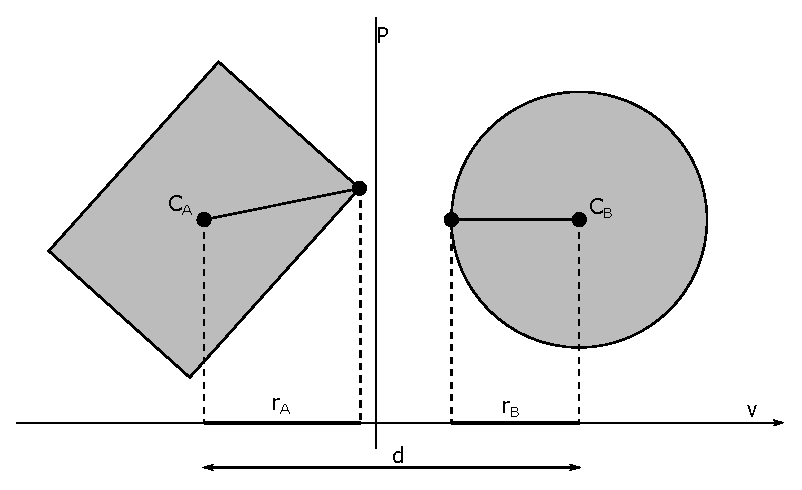
\includegraphics[width=\textwidth]{pics/cap3_01.eps}
		\label{fig:cap3_01}
		\caption{hiperplanul de separație $P$, axa separatoare $v$ și razele de proiecție $r_A$ și $r_B$ ale două corpuri care nu se intersectează}
		\vfill
	\end{subfigure}
	\hfill
	\begin{subfigure}[t]{0.49\textwidth}
		\centering
		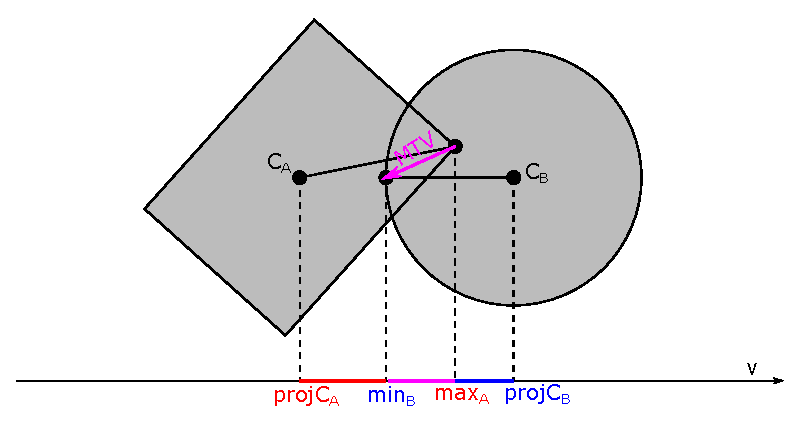
\includegraphics[width=\textwidth]{pics/cap3_02.eps}
		\label{fig:cap3_02}
		\caption{o axă arbitrară $v$ și vectorul minim de translație $MTV$(eng. \textit{minimum translation vector}) pentru această axă în cazul unei intersecții}
	\end{subfigure}
	\caption{Teorema axei separatoare}
\end{figure}
Astfel, două obiecte nu se intersectează(pe o axă) dacă suma razelor lor de proiecție este mai mică decât distanța dintre proiecțiile centrelor lor pe acea axă. În cazul poliedrelor convexe, intersecția poate fi de 3 tipuri: față-față, față-muchie, muchie-muchie (vârfurile pot fi considerate muchii degenerate) și este suficient să testăm doar următoarele posibile axe de separare:
\begin{itemize}
	\item axele paralele cu normalele fețelor obiectului A
	\item axele paralele cu normalele fețelor obiectului B
	\item axele paralele cu vectorii rezultați în urma produsului vectorial al tuturor muchiilor lui A cu toate muchiile lui B
\end{itemize}
Normala de coliziune este chiar axa care a rezultat într-o penetrare minimă, distanța de separare este chiar lungimea vectorului minim de translație ($min_B - max_A$ sau $min_A - max_B$), iar pentru determinarea punctelor de contact, se vor calcula pentru ambele obiecte, \hyperref[support_points]{punctele suport} în direcția de separare.


\textbf{Algoritmul Gilbert-Johnson-Keerthi}(GJK) este o altă metodă de a determina cu precizie dacă două obiecte se intersectează. A fost propus inițial în 1988\cite{gjk_original}, ca metodă de a determina distanța euclidiană între două mulțimi convexe din $\mathbb{R}^n$, iar o implementare eficientă și robustă a fost propusă de Gino van den Bergen în 1998\cite{gjk_gino}.
\begin{algorithm}[H]
	\footnotesize
	\linespread{0.9}\selectfont
	\caption{Testul de intersecție Gilbert-Johnson-Keerthi}
	\label{gjk_intersection_test}
	\begin{algorithmic}[0]
		\Function {GJKTestIntersection}{$shape\_A$, $shape\_B$, $init\_dir$}
			\State $new\_point \gets \textproc{Support}(shape\_A, init\_dir) - \textproc{Support}(shape\_B, -initial\_dir)$
			\State $simplex \gets \left\lbrace new\_support\_point \right\rbrace $
			\State $dir \gets -new\_point$
			\Loop
				\State $new\_point \gets \textproc{Support}(shape\_A, dir) - \textproc{Support}(shape\_B, -dir)$
				\If{$\textproc{dot}(new\_point, dir) < 0$}
					\State $\textbf{return}\ False$
				\EndIf
				\State $simplex \gets simplex\ \cup\ new\_point $
				\State $simplex, dir, contains\_origin \gets \textproc{DoSimplex}(simplex) $
				\If{$contains\_origin$}
					\State $\textbf{return}\ True$
				\EndIf
			\EndLoop
		\EndFunction
		\Statex
		\Function {DoSimplex}{$simplex$}
			
			1. determină simplex-ul cel mai apropiat de origine care se poate forma din cât mai puține din punctele simplex-ului dat ca parametru
			
			2. direcția de căutare devine normala către origine a noului simplex
			
			3. în cazul tetraedru, întoarce True dacă simplex-ul conține originea
		\EndFunction
	\end{algorithmic}
\end{algorithm}

Practic, la fiecare iterație, \hyperref[simplex]{simplex-ul} încearcă să se extindă și să cuprindă originea, adăugând mereu un punct suport de pe \hyperref[minkowski_difference]{diferența Minkowski} a celor două obiecte, aflat în direcția originii, până când aceasta este cuprinsă în simplex sau nu se mai apropie de acesta.



În cazul în care algoritmul GJK a stabilit că există o coliziune, pentru determinarea normalei, distanței de penetrare și a punctelor de contact, \textbf{algoritmul EPA}\cite{epa_gino}(eng. \textit{expanding polytope algorithm}) este continuarea firească. Acesta preia \hyperref[simplex]{simplex-ul} rezultat în urma aplicării GJK și îl extinde iterativ cu \hyperref[support_points]{puncte suport} de pe frontiera \hyperref[minkowski_difference]{diferenței Minkowski}, până când distanța minimă dintre politopul rezultat și origine nu se mai modifică. Odată întâlnită această situație, \hyperref[barycenric_coordinates]{coordonatele baricentrice} ale proiecției originii pe triunghiul(în cazul 3D) sau dreapta(în cazul 2D) cele mai apropiate de origine pot fi folosite pentru determinarea punctelor de contact, iar distanța de la origine la triunghi(sau dreaptă) este chiar distanța de penetrare și normala contactului. Expansiunea politopului se face prin divizarea feței celei mai apropiate și crearea de noi triunghiuri sau laturi folosind punctul nou ales și punctele rămase.

\begin{algorithm}[]
	\footnotesize
	\linespread{0.9}\selectfont
	\caption{Expanding Polytope Algorithm și determinarea punctelor de contact}
	\label{epa}
	\begin{algorithmic}[0]
		\Function {EPACreateContact}{$shape\_A$, $shape\_B$, $simplex$}
			\State $ polytope \gets simplex.triangles $
			\Loop
				\State $ closest\_triangle \gets \argmin_tr \textproc{distance}(tr, origin), tr \in polytope $
				\State $ distance \gets \textproc{distance}(closest\_triangle, origin) $
				\State $ normal \gets closest\_triangle.normal $
				\State $ new\_point \gets \textproc{Support}(shape\_A, normal) - \textproc{Support}(shape\_B, -normal) $
				\State $ new\_distance \gets \textproc{distance}(new\_point, origin) $
				\If{$ new_distance - distance < threshold $}
					\State $ coords \gets \textproc{barycentric}(origin, closest\_triangle) $
					
				\State	$ contact\_points \gets $ pentru fiecare obiect, se calculează punctul de contact în funcție de corespondențele fiecărui punct al triunghiului din mulțimea de puncte a obiectului respectiv
				\State $ \textbf{return}\ contact\_points, normal, distance $
				\EndIf
				\State $ polytope \gets polytope \setminus \left\lbrace closest\_triangle \right\rbrace $
				\State creează triunghiuri noi folosind $ new\_point $ în spațiul lăsat descoperit
			\EndLoop
		\EndFunction
	\end{algorithmic}
\end{algorithm}

\subsection{Rezolvare coliziuni}
În esență, rezolvarea coliziunilor implică aplicarea unui \textbf{răspuns} asupra corpurilor aflate în contact, care să conducă la separarea acestora. În lumea reală, răspunsul vine sub forma forțelor elastice care se opun comprimării(oricât de mică ar fi aceasta) corpurilor aflate în contact, care determină o accelerație care reduce viteza de ciocnire până la valori negative, când corpurile se separă. În cadrul unui motor de fizică, acest fenomen este simulat cu ajutorul \textbf{impulsurilor} -- modificări bruște a vitezelor obiectelor aflate în coliziune, astfel încât acestea să tindă spre separare. În general, sunt suficiente două impulsuri -- cel liniar și cel unghiular, fiecare modificând viteza corespondentă.

Soluționarea unei coliziuni este de regulă realizată cu ajutorul conceptului mult mai general de \textbf{constrângeri fizice}, definite ca o serie de ecuații și inecuații care trebuie să fie satisfăcute. În cazul rezolvării unei coliziuni, constrângerea care trebuie satisfăcută de vitezele celor două corpuri este:
$$ \dot{C} \colon \left( -\vec{V_A} - \vec{\omega_A} \times \vec{r_A} + \vec{V_B} + \vec{\omega_B} \times \vec{r_B} \right) \cdot \vec{n} + b\geq 0 $$unde:
\begin{itemize}
	\item $\vec{V_A}, \vec{V_B}$ sunt vitezele liniare ale celor două corpuri
	\item $\vec{\omega_A}, \vec{\omega_B}$ sunt vitezele unghiulare ale celor două corpuri
	\item $\vec{r_A}, \vec{r_B}$ sunt definite ca $P_A - C_A$ și $P_B - C_B$, cu $P_A,P_B$ punctele cele mai adânci de interpenetrare și $C_A, C_B$ centrele de masă ale corpurilor
	\item $\vec{n}$ este normala contactului
	\item $b$ este un termen de bias, care corespunde vitezei de separare a celor două corpuri și este influențat de coeficientul de restituire al ciocnirii: $$b = C_R\left( -\vec{V_A} - \vec{\omega_A} \times \vec{r_A} + \vec{V_B} + \vec{\omega_B} \times \vec{r_B} \right) \cdot \vec{n} $$
\end{itemize}

Frecările sunt rezolvate sub forma unor \textbf{impulsuri tangențiale}, care vor modifica viteza corpurilor în două direcții perpendiculare pe normala de contact, în plus față de \textbf{impulsul normal}.

La calculul impulsurilor se ține cont și de masele celor două corpuri și de \hyperref[inertia_tensor]{tensorii de inerție}. O derivare a formulei poate fi urmărită în prezentarea lui Erin Catto\cite{constraints_catto}.


O simulare va conține un număr mare de contacte, care se pot afecta unele pe altele(de ex. în cazul unei stive de obiecte), motiv pentru care rezolvarea acestora se face iterativ, până la convergență. Astfel, dacă rezolvarea unui contact va afecta un altul (este modificată distanța de penetrare, normala sau viteza de întâlnire), acest lucru se va reflecta în iterațiile succesive și sistemul poate găsi soluția corectă. În realitate, într-o simulare, acest lucru se întâmplă destul de rar, dar rezultatele obținute sunt satisfăcătoare, imperfecțiunile fiind neglijabile.

Realistic vorbind, o coliziune este deseori formată din mai multe puncte de contact, care împreună formează un \textbf{manifold} care trebuie rezolvat.
\begin{figure}[H]
	\centering
	\includegraphics[width=0.7\linewidth]{pics/cap3_03.png}
	\label{fig:cap3_03}
	\caption[]{3 cazuri de contact și manifold-urile lor}
\end{figure}
În acest scop, există 2 posibile abordări \cite[Secțiunea 6.6.2~\textit{Collision response for colliding contact}]{game_physics_eberly}:
\begin{enumerate}
	\item \textbf{Metoda impulsurilor secvențiale} -- impulsurile sunt calculate și aplicate iterativ în fiecare dintre punctele de contact.
	\item \textbf{Metoda contactelor simultane} -- Jacobian-ul folosit pentru calculul impulsurilor este determinat pe baza tuturor punctelor din manifold-ul de contact, iar impulsurile sunt aplicate o singură dată per manifold.
\end{enumerate}

\subsection{Integrare numerică}
Într-un motor de fizică, etapa de integrare constă în actualizarea stării obiectelor, prin \textbf{integrarea în raport cu timpul} a mărimilor fizice derivate. Ne amintim de la orele de fizică din liceu că accelerația unui corp este dată de formula $ a = \frac{F}{m} $, unde $F$ este rezultanta forțelor care acționează asupra corpului și $m$ este masa acestuia. Într-o simulare, accelerația este considerată o mărime fizică primară și este cea dintâi calculată în fiecare cadru. Accelerația este totodată definită și ca variația vitezei în timp, iar viteza este variația poziției în timp, ceea ce ne permite să calculăm atât viteza $\dot{p}'$, cât și poziția $p'$, prin integrarea accelerației $\ddot{p}$, respectiv vitezei $\dot{p}$:
$$ \dot{p}' = \dot{p} + \ddot{p}t $$
$$ p' = p + \dot{p}t + \ddot{p}\frac{t^2}{2} \approx p + \dot{p}t $$
Deoarece într-o simulare avem de-a face cu momente discrete de timp(dictate de diferența de timp dintre două cadre -- \textbf{deltaTime}, aceste valori trebuie aproximate, de unde rezultă nevoia folosirii unor metode de integrare numerică cu pas de timp discret.
Se disting o serie de metode, mai mult sau mai puțin precise\cite{integration_gaffer}:
\begin{itemize}
	\item \textbf{Metoda Euler explicită} presupune determinarea, în ordine, mai întâi a noii poziții și apoi a noii viteze, dar are dezavantajul că pierde din precizie dacă există variații mari ale mărimilor de la un cadru la altul, cu eroare de ordinul $O(deltaTime)$
	\begin{lstlisting}[style=myC++]
		position = position + velocity * deltaTime;
		velocity = velocity + acceleration * deltaTime;
	\end{lstlisting}
	\item \textbf{Metoda Euler semi-implicită} presupune folosirea noii viteze la determinarea noii poziții și este considerabil mai precisă, cu eroare de ordinul $O(deltaTime^2)$
	\begin{lstlisting}[style=myC++]
	velocity = velocity + acceleration * deltaTime;
	position = position + velocity * deltaTime;
	\end{lstlisting}
	\item \textbf{Metoda Runge-Kutta 4} evaluează derivata stării în 4 puncte diferite din cadrul intervalului de derivare, folosind ca feedback rezultatele anterioare și este mult mai precisă, ceea ce conduce la o eroare de ordinul $O(deltaTime^4)$
\end{itemize}

\subsection{Interfață grafică}
TODO:
\section{Alegeri pentru lucrarea de față}

Dintre soluțiile menționate în subsecțiunile de mai sus, am fost nevoit să fac niște alegeri, pe care urmează să le prezint și să le motivez în continuare.

\subsection{Detecție coliziuni}

Deoarece scenele cu care am testat simulatorul sunt de dimensiuni relativ mici(sub 100 de obiecte), am decis că o ierarhie de volume încadratoare nu aduce o îmbunătățire semnificativă în raport cu overhead-ul pe care l-ar aduce etapei de implementare a soluției. La fel, o partiționare a spațiului scenei în arbori, folosind BSP mi s-a considerat nejustificată. Astfel, m-am utilizat doar de un \textbf{detector $O(n^2)$}, care testează intersecția dintre \textbf{OBB-urile} obiectelor folosind \textbf{Teorema axei separatoare}.

Pentru că obiectele din scenă sunt doar corpuri geometrice elementare pentru care nu stochez liste de vârfuri, muchii și fețe, ci doar descrierea geometrică a formei acestora, Teorema axei separatoare nu se pretează pentru determinarea punctelor de contact. În plus, corpurile rotunde(cilindru, con, sferă, capsulă) ar pune probleme în realizarea testului de separare, deoarece ar avea nevoie de un număr foarte mare de axe care să fie testate. În schimb, am ales să folosesc \textbf{algoritmul GJK}, care se poate folosi de descrierea geometrică a formei corpurilor pentru calculul facil al punctelor de suport necesare la determinarea simplex-ului final.

Și, în mod evident, algoritmul GJK se potrivește de minune cu \textbf{EPA}, având în comun o bună parte dintre metode și structuri de date.

\subsection{Rezolvare coliziuni}

Complexitatea pe care ar fi adus-o implementarea metodei rezolvării simultane a contactelor nu este justificată în cazul de față. Ar fi fost nevoie de un redesign al structurilor de date folosite adus de necesitatea operațiilor dintre matrice și vectori de dimensiuni mari, direct proporționale cu numărul de contacte din manifold -- ar fi trebuit să îmi scriu propria implementare pentru structurile geometrice de date - vectori și matrice de dimensiuni mai mari decât 4x4. Am ales, astfel, să utilizez \textbf{metoda impulsurilor secvențiale}, care produce rezultate acceptabile pentru o simulare care nu se vrea a fi hiper-exactă.

De asemenea, am decis să nu generalizez contactele la constrângeri fizice și am ales să introduc în schimb alte optimizări, descrise în capitolele ulterioare.

\subsection{Integrare numerică}

În cazul unei simulări, metoda Euler explicită este inferioară din toate punctele de vedere celei \textbf{Euler implicită}, iar precizia altor metode de ordin superior ar fi combătute oricum de micile imperfecțiuni apărute în urma rezolvării coliziunilor. Am ales să păstrez lucrurile simple și să folosesc a doua metodă prezentată mai sus.
% 
%\dezvoltare Ce soluții similare există pe piață? Care sunt limitările lor / pentru ce cazuri de utilizare sau pentru ce tip de clienți produsele existente pe piață nu răspund cerințelor? Care sunt indicatorii pe baza cărora sunt evaluate aceste produse, de către potențiali clienți, și unde sunt lipsurile/ care este oportunitatea generată de lipsurile acestea?
%
%\cercetare Metode existente (sau ``State of the Art'') se referă, de regulă, la nivelul curent de dezvoltare: care este starea curentă a domeniului, unde ne găsim, care este contextul. Care sunt soluțiile actuale prezente în literatura de specialitate și care sunt limitările lor? Ce direcții de explorare sunt recomandate în literatura de specialitate? Literatura de specialitate se refera la articole științifice recente, publicate în reviste cu factor de impact mare, sau în volumele unor conferințe de top, sau în cărți.
%
%\ambele În încheierea acestui capitol se dorește descrierea tehnologiilor folosite în lucrare, cu alternative și cu argumente convingătoare calitative și cantitative.  
%
%Criterii pentru calificativul \textit{Ne\textit{Satisfăcător}}: 
%\begin{itemize}
%	\item \dezvoltare Sunt analizate superficial câteva produse de pe piață; 
%	\item \cercetare analiza literaturii limitata la grupuri de cercetare din România;
%	\item \ambele Sunt descrise tehnologiile folosite în lucrare. 
%\end{itemize}
%
%Criterii pentru calificativul \textit{Satisfăcător}:
%\begin{itemize}
%	\item \dezvoltare Există un interviu, un client, analiza cerințelor este elaborată pe baza interviului.
%	\item \cercetare analiza literaturii de specialitate din lume, fără poziționarea precisă a lucrării în peisajului domeniului studiat;
%	\item \ambele Sunt descrise câteva tehnologii alternative pentru fiecare din tehnologiile folosite în lucrare. Există o argumentare referitoare la alegere.
%\end{itemize}
%
%Criterii pentru calificativul \textit{Bine}:
%\begin{itemize}
%	\item \dezvoltare Proces iterativ pe baza unor interviuri cu mai mulți clienți, dezvoltare MVP, reevaluare cerințe;
%	\item \cercetare analiza literaturii de specialitate din lume, cu poziționarea precisă a lucrării în peisajul actual al domeniului studiat; 
%	\item \ambele Sunt descrise tehnologii alternative. Sunt analizate cantitativ și calitativ, folosite benchmarkuri și teste efectuate de student. Analiza este rezumată prin tabele și grafice.
%\end{itemize}
%
%\section{Indicații formatare figuri}
%
%Figurile utilizate în document vor fi centrate și numerotate (de exemplu Figura~\ref{fig:pic1}). 
%Orice figură ce nu este realizată de către autorul lucrării va fi în mod obligatoriu citată fie la final (de exemplu Figura ~\ref{fig:pic2} este preluată din documentul \cite{}), fie cel puțin într-o notă de subsol (a se vedea Figura~\ref{fig:pic2}). Orice figură ce depășește ca dimensiune 50\% dintr-o pagină, va fi mutată la anexe. Toate figurile din cadrul tezei vor fi referite în text. Exemplu: Figura~\ref{fig:pic1} prezintă o schemă de principiu pentru un amplificator inversor cu AO. 
%
%\begin{figure}[th]
%\centering
%\includegraphics{pics/Pic1.png}
%  \caption{Amplificator inversor}
%  \label{fig:pic1}
%\end{figure}
%
%\newpage
%
%\begin{figure}[th]
%\centering
%\includegraphics{pics/Pic2.png}
%  \caption[Amplificator de instrumentație cu 3 AO-uri]{Amplificator de instrumentație cu 3 AO-uri\protect\footnotemark}
%  \label{fig:pic2}
%\end{figure}
%\footnotetext{© http://www.ece.tamu.edu/sspalermo/ecen3205/Secton\%201III.pdf}

\chapter{Soluția Propusă}

Soluția propusă urmărește arhitectura firească a unei aplicații grafice \textbf{OpenGL}, cu următoarele componente:

\begin{enumerate}
	\item \textbf{backend}-ul -- este un framework care oferă funcționalitățile de bază necesare funcționării aplicației OpenGL
	\item \textbf{logica} -- este implementarea propriu-zisă a simulatorului de interacțiuni fizice
	\item \textbf{frontend}-ul -- reprezintă interfața cu utilizatorul
\end{enumerate}

\section{Backend-ul}

Funcționalitățile pe care le oferă așa-numitul backend sunt:
\begin{itemize}
	\item crearea, controlul și interfațarea cu un context OpenGL
	\item suport pentru încărcarea de meshe 3D
	\item suport pentru definirea și încărcarea de shadere OpenGL
	\item crearea și controlul unei ferestre de afișare
	\item oferirea unui model generic pentru scrierea de aplicații OpenGL:
		\begin{itemize}
			\item control pentru fereastra de afișare
			\item management-ul input-ului de la mouse și tastatură
			\item implementarea unei camere first-person pentru vizualizarea scenei
			\item o scenă de bază care poate fi moștenită și căreia i se vor adăuga funcționalitățile specifice aplicației
			\item interfață pentru desenarea meshelolor 3D
		\end{itemize}
\end{itemize}
Lista de mai sus nu este exhaustivă, complexitatea unui astfel de framework, chiar și minimal, este destul de mare. Cum implementarea acestuia nu a făcut parte din obiectivele proiectului, am ales să folosesc framework-ul realizat de Gabriel Ivănică pentru laboratoarele de EGC\cite{framework_egc_github}. O descriere mai detaliată a acestuia poate fi găsită aici\cite{framework_egc_ocw}.

Astfel, etapele funcționării unei aplicații, facilitate de framework-ul descris mai sus sunt:
\begin{enumerate}
	\item Se definesc proprietățile pentru fereastra de lucru.
	\item Se inițializează API-ul OpenGL.
	\item Se creează fereastra de lucru cu un context OpenGL.
	\item Se atașează evenimentele de fereastră la motorul care se ocupă de tratarea lor.
	\item Se creează și se inițializează noua scenă 3D.
	\item Se pornește bucla principală a aplicației.
\end{enumerate}

\section{Logica aplicației}

Este componenta centrală a oricărei aplicații grafice și funcționează în întregime în cadrul buclei principale de program.

\subsection{Funcționare}
Într-o iterație au loc următorii pași:
\begin{enumerate}
	\setcounter{enumi}{-1}
	\item Backend-ul realizează un preambul în care își actualizează parametrii interni
	\begin{itemize}
		\item Se pregătește contextul OpenGL pentru desenare -- sunt curățate buffer-ele de culoare, dimensiunea ferestrei de desenare este reactualizată, dacă este cazul
		\item Se estimează timpul de execuție pentru iterația actuală, pe baza duratei iterației precedente(deltaTime).
		\item Sunt procesate evenimentele salvate anterior.
	\end{itemize}
	\item Este desenată scena în totalitate.
	\item Se actualizează starea obiectelor din simulare, prin efectuarea pasului de integrare.
	\item Se efectuează faza preliminară a detecției de coliziuni -- se obține o listă de perechi de obiecte posibil aflate în contact.
	\item Se efectuează faza exactă a detecției de coliziuni -- lista de mai sus este prelucrată și sunt actualizate vechile contacte, în cazul perechilor de obiecte aflate în coliziune continuă, sau sunt generate altele noi.
	\item Se încearcă, iterativ, rezolvarea tuturor contactelor din scenă.
	\item Se face trecerea la următorul cadru -- se revine la pasul 0.
\end{enumerate}
\begin{itemize}
	\item Pentru a nu bloca execuția simulării, toate evenimentele de input sau de control al ferestrei sunt salvate de backend într-un buffer, pentru a putea fi soluționate toate deodată în pasul 0.
\end{itemize}

\subsection{Structură}
În continuare voi descrie, pe rând, componentele individuale ale simulatorului.

\begin{figure}[H]
	\centering
	\includegraphics[width=0.4\linewidth]{pics/cap4_00.eps}
	\label{fig:physicsObject}
	\caption[]{Descrierea unui obiect al scenei}
\end{figure}

Începând cu \textbf{obiectele scenei}, acestea sunt alocate dinamic la rularea aplicației și stochează informații necesare la desenare, dar oferă și o interfață pentru actualizarea corpului solid, prin metoda \textbf{update()}. Am ales să folosesc obiectul scenei ca pe o scurtătură către toate referințele necesare celorlalte componente(de ex. în cadrul algoritmului GJK, determinarea punctului de suport pe diferența Minkowski a 2 corpuri necesită apelul metodei \textit{getSupportPtInLocalSpace()} din clasa Shape și poate fi accesată prin referința din PhysicsObject).

Starea cinematică a obiectului este încapsulată într-un obiect \textbf{RigidBody}(descris în întregime aici \ref{fig:RigidBody}). Pasul de integrare presupune:
\begin{enumerate}
	\item \textbf{determinarea accelerației} ca rezultat al forțelor care acționează asupra obiectului
	\item determinarea noilor valori pentru \textbf{viteză}(atât liniară, cât și unghiulară), și pentru \textbf{poziție}, respectiv \textbf{orientare}, folosind metoda Euler semi-implicită
	\item sunt simulate forțele de frecare cu aerul, prin înmulțirea vitezelor cu un \textbf{factor de amortizare}
	\item sunt actualizate \textbf{matricele de modelare} și \textbf{tensorul de inerție} și se resetează acumulatorii de forțe și momente 
\end{enumerate}

Mai departe, controlul aplicației este preluat de \textbf{detectorul de coliziuni}, a cărui structură completă poate fi găsită aici \ref{fig:CollisionDetection}.

\begin{figure}[H]
	\centering
	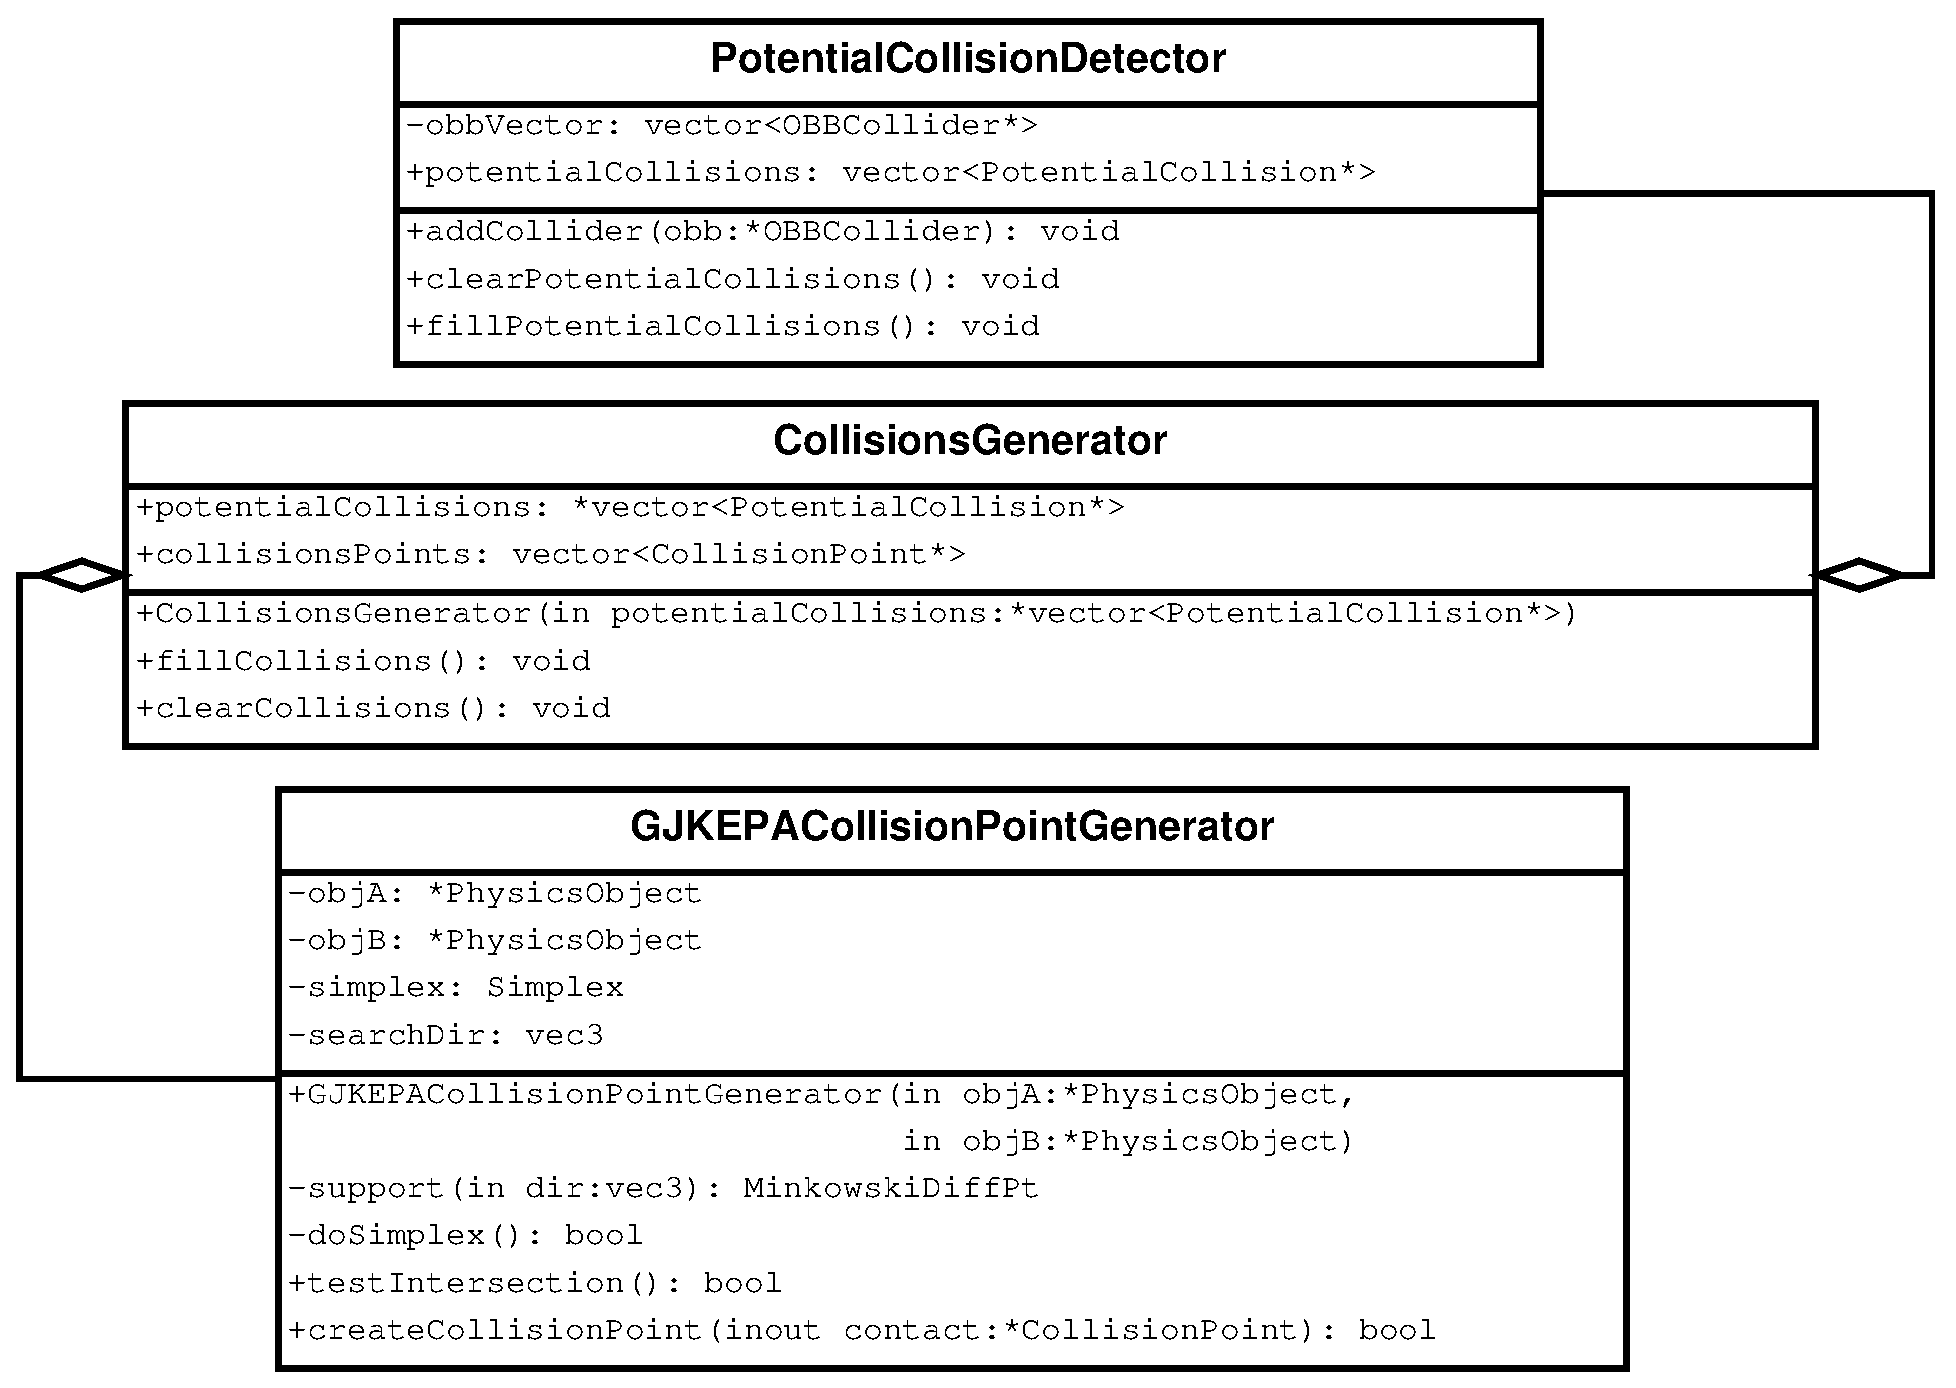
\includegraphics[width=0.8\linewidth]{pics/CollisionDetectionSmall.eps}
	\caption[]{Sistemul de detecție de coliziuni}
	\label{fig:CollisionDetectionSmall}
\end{figure}

Am considerat necesară separarea procesului de detecție a coliziunilor în două subsisteme -- \textbf{detectorul de posibile coliziuni}, corespondent fazei preliminare a algoritmului și \textbf{generatorul de puncte de coliziune}, care preia responsabilitatea pentru corpurile descoperite de primul. \textbf{generatorul de coliziuni} nu este decât un agregator al celor două subsisteme care oferă o interfață simplă aplicației.

\begin{figure}[H]
	\centering
	\includegraphics[width=0.7\linewidth]{pics/collider.eps}
	\caption[]{OBBCollider implementează clasa abstractă Collider}
	\label{fig:collider}
\end{figure}

Detectorul de posibile coliziuni menține un \textbf{vector de collider-e OBB} pentru obiectele din scenă pentru care se dorește posibilă existența coliziunilor și construiește \textbf{vectorul de posibile coliziuni} folosind referințele către obiectele fizice din collider-e. Generatorul de puncte de coliziune preia rezultatul și efectuează, mai întâi testul de intersecție, și mai apoi calculează punctele de coliziune, care este rezultatul final al etapei de detecție a coliziunilor și care este transmis mai departe în pipeline \textbf{rezolvitorului de coliziuni}.

Deoarece \textbf{punctele de coliziune} reprezintă doar niște informații legate de coliziunea cea mai adâncă dintre 2 corpuri(câte un singur punct pe suprafețele celor două corpuri, normala și distanța de penetrare) și ar fi ineficient să se aloce dinamic noi contacte la fiecare cadru, am folosit o schemă de caching bazată pe ideea de \textbf{contacte persistente} și \textbf{manifold-uri de contact}:
\begin{itemize}
	\item introduc aici noțiunea de \textbf{punct de contact}, care pe lângă informațiile de coliziune, mai include și alte câmpuri necesare algoritmului de caching sau rezolvării în sine
	\begin{figure}[H]
		\centering
		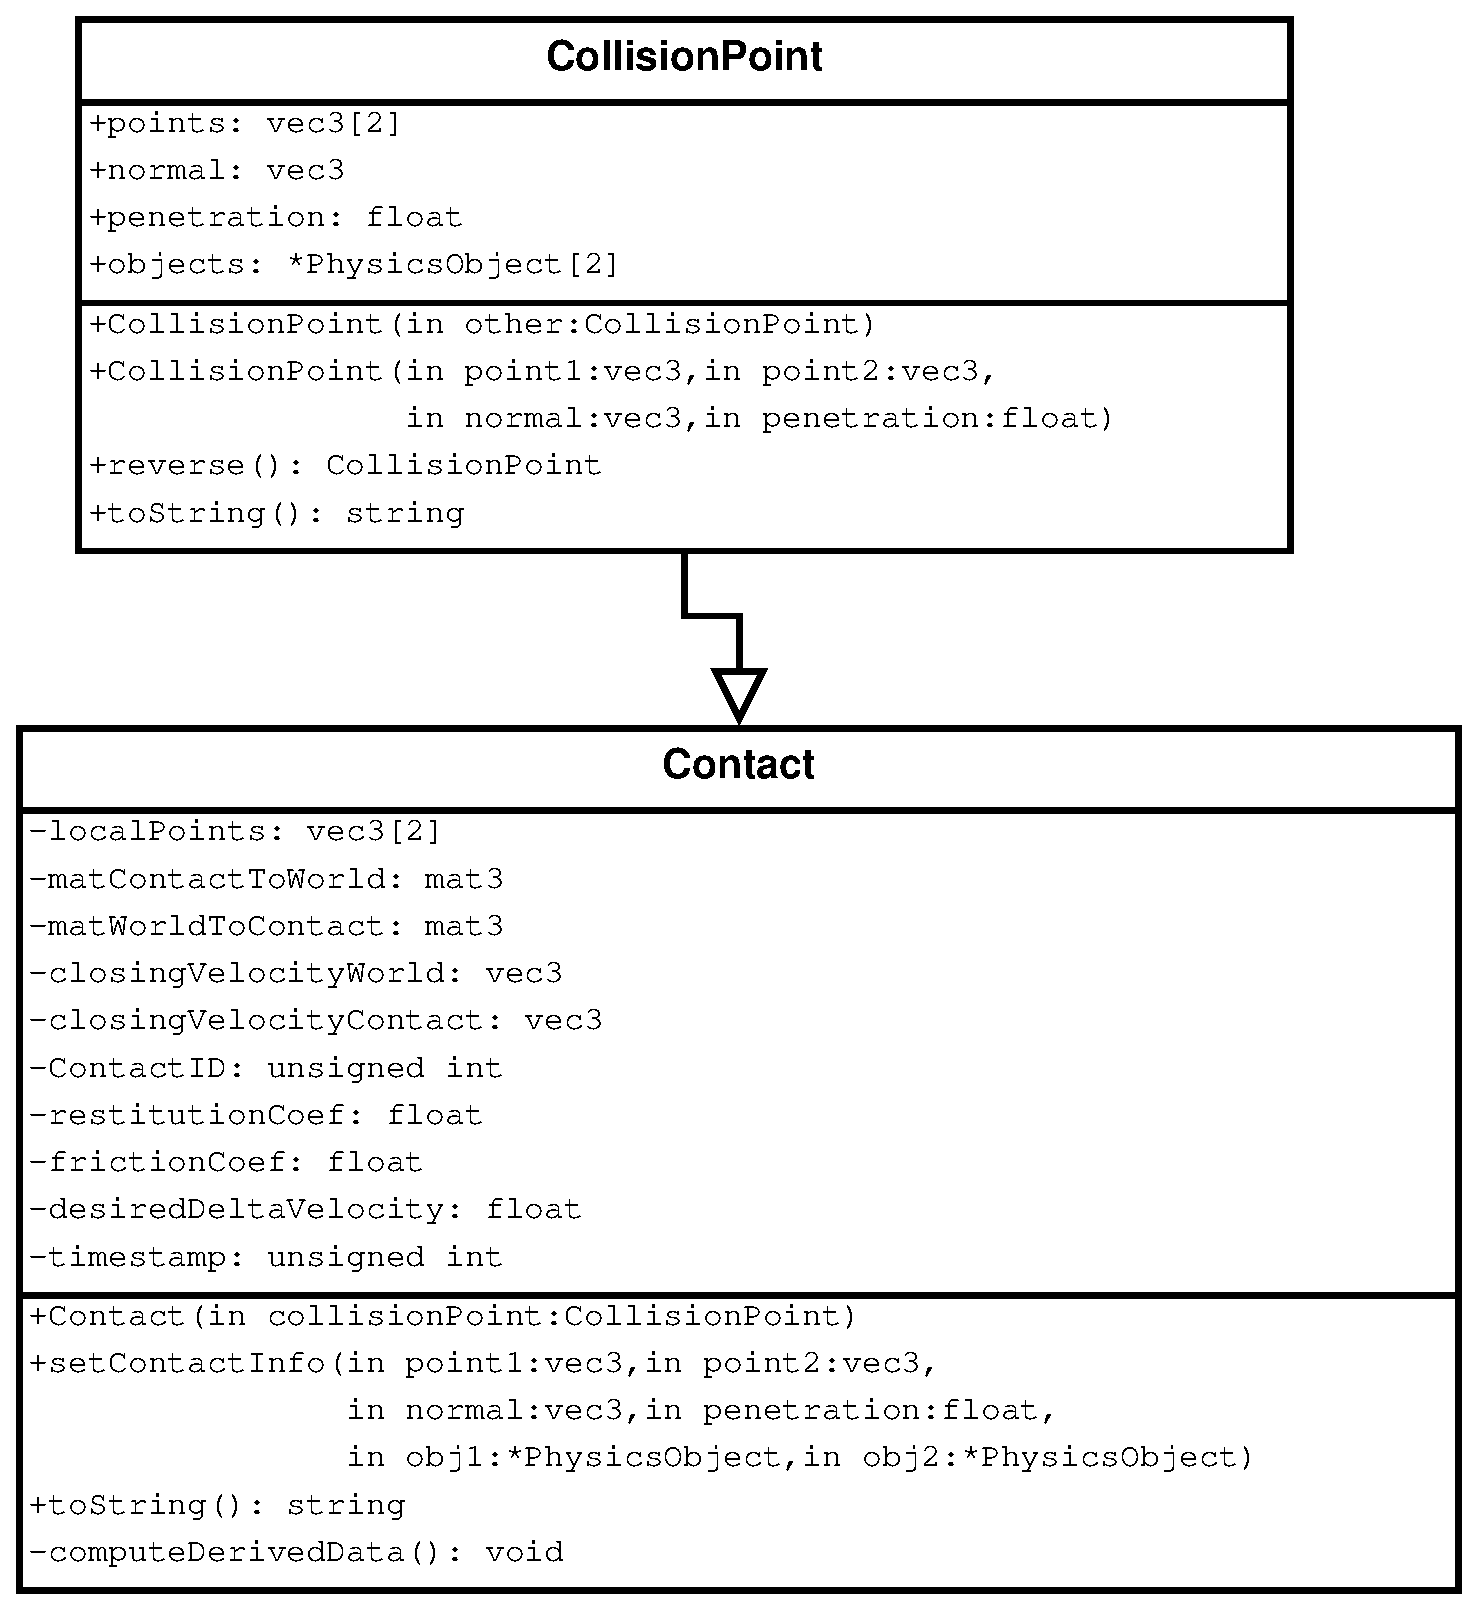
\includegraphics[width=0.7\linewidth]{pics/collisionContact.eps}
		\caption[]{\centering diferența subtilă dintre punctul de coliziune și punctul de contact \newline (a se observa că Contact moștenește CollisionPoint)}
		\label{fig:collisionContact}
	\end{figure}
	\item pentru fiecare pereche de obiecte pentru care există coliziune, punctele de contact sunt reținute într-un manifold format din maxim 4 astfel de puncte
	\item de fiecare dată când obțin un nou punct de coliziune între două obiecte, caut manifold-ul de contact asociat perechii de obiecte și îl actualizez:
	\begin{itemize}
		\item dacă nu am găsit un manifold pentru perechea curentă, atunci creez unul nou și creez un nou punct de contact pe care îl adaug la manifold
		\item dacă punctul de coliziune poate fi atribuit unuia dintre punctele de contact ale manifold-ului(se află la o distanță suficient de mică), atunci doar actualizez punctul de contact deja existent
		\item dacă nu corespunde unui astfel de punct, atunci este creat un nou punct de contact și este adăugat manifold-ului, înlocuind, dacă există deja 4 puncte, punctul de contact care oferă cea mai puțină informație(cel cu penetrarea cea mai mică)
	\end{itemize}
	\item manifold-urile care nu au fost actualizate în cadrul curent, sau cele formate din puncte de contact cu penetrare negativă, sunt pur și simplu eliminate din sistem
\end{itemize}

Cu asta se încheie pipeline-ul logic al simulatorului. Totul se reia de la început în noul cadru.

\section{Interfața cu utilizatorul}
TODO:
%Capitolul conține o privire de ansamblu a soluției ce rezolvă problema, prin prezentarea structurii / arhitecturii acesteia. În funcție de tipul lucrării acest capitol poate conține diagrame (clase, distribuție, workflow, entitate-relație), demonstrații de corectitudine pentru algoritmii propuși de autor, abordări teoretice (modelare matematică), structura hardware, arhitectura aplicației.
%
%
%Criterii pentru calificativul \textit{Ne\textit{Satisfăcător}}: 
%\begin{itemize}
%	\item	Descriere în limbaj natural.
%\end{itemize}
%
%Criterii pentru calificativul \textit{Satisfăcător}: 
%\begin{itemize}
%	\item	Descriere + diagrame de baze de date, workflow, clase, algoritmi. 
%\end{itemize}
%
%Criterii pentru calificativul \textit{Bine}: 
%\begin{itemize}
%	\item 	Descriere + diagrame de baze de date, workflow, clase, algoritmi + descrierea unui proces prin care s-a realizat arhitectura/structura soluției.
%\end{itemize}
%
%\section{Indicații formatare formule}
%Formulele matematice utilizate în document vor fi centrate în pagină și numerotate. 
%
%\begin{equation}
%(x+a)^n = \sum_{k=0}^{n}\left(\begin{array}{c}n\\k\\\end{array}\right)x^ka^{n-k}
%\end{equation}
%
%\begin{equation}
%f(x) = a_0 + \sum_{n=1}^{\infty}\left(a_n \cos\frac{n\pi x}{L} + b_n\sin\frac{n\pi x}{L}\right)
%\end{equation}



\chapter{Detalii de implementare}

Acest capitol conține câteva observații asupra procesului de dezvoltare și implementare a aplicației aferente proiectului.

Implementarea a fost realizată folosind limbajul \textbf{C++} și biblioteca \textbf{OpenGL}, în mediul de programare Microsoft \textbf{Visual Studio} Community Edition 2017, iar testarea s-a făcut pe laptop-ul personal(Intel i5 2.5GHz, 8GB RAM, Intel HD Graphics 4600).

Dezvoltarea a pornit de la framework-ul utilizat la laboratoarele de EGC, care a fost descris în capitolul precedent. Acesta oferă clasa abstractă SimpleScene, care poate fi moșteniță și care oferă interfețe pentru rularea aplicației(metodele Init(), FrameStart(), Update(), FrameEnd()), randarea de meshe și pentru tratarea de input de la mouse și tastatură. Aplicațiile demo sunt pur și simplu implementări ale acestei SimpleScene. În plus, framework-ul oferă și implementarea unei camere first-person, care poate fi controlată din mouse și tastatură, pentru vizualizarea scenei.

Biblioteca folosită pentru tipuri și funcții matematice și geometrice este \textbf{GLM}


Primul obiectiv atins a fost \textbf{implementarea clasei RigidBody}\ref{fig:RigidBody} și, implicit, a operației de integrare. Testarea s-a făcut cu un simplu cub asupra căruia acționează gravitația și asupra căruia se pot aplica forțe, momente și impulsuri cu ajutorul tastaturii. Singura mențiune specială este că am ales să stochez orientarea corpului într-un \textbf{quaternion}, în loc de o reprezentare matriceală sau cu unghiurile lui Euler. Motivul este foarte simplu, ocupă mai puțin spațiu în memorie, nu prezintă problema Gimbal Lock\cite{quaternions}, iar suportul GLM pentru operații cu quaternioni este foarte bun. Exemplu de utilizare:
\begin{lstlisting}[style=myC++]
	glm::quat orientation;
	...
	orientation = orientation + deltaTime * 0.5f * glm::quat(0.0f, angVelocity) * orientation;
	orientation = glm::normalize(orientation);
\end{lstlisting}


A doua etapă de dezvoltare a constat în implementarea sistemului de \textbf{detecție a coliziunilor}. Complexitatea etapei mi-a pus mult mai multe bătăi de cap.

Pentru \textbf{faza preliminară}, am implementat direct collider-ele de tip OBB, cu un detector $O(n^2)$. După ce am citit despre teorema axei separatoare și eșuarea în a corecta erorile din implementarea mea a testului de intersecție, am ales să folosesc cea mai eficientă implementare posibilă, cea propusă de Ericson în \cite[Secțiunea 4.4 \textit{Oriented Bounding Boxes(OBBs)}]{real_time_collision_detection}. Tot aici, am fost nevoit să implementez abstractizarea obiectelor din scenă, care să încapsuleze obiectele RigidBody și Collider.

Faza de detecție exactă și generare a punctelor de coliziune este cea care mi s-a părut cea mai dificilă. A necesitat o foarte mare atenție la detalii cum ar fi ordinea vârfurilor care compun simplex-ul din algoritmul GJK sau triunghiurile care compun poliedrul din cadrul EPA. Pentru implementarea GJK, foarte utilă mi s-a părut explicația lui Casey Muratori\cite{gjk_muratori}, care a oferit o interpretare mult mai ușor de înțeles a algoritmului decât enunțarea lui inițială\cite{gjk_original}. Remarcabil mi se pare că în cazul unui simplex tetraedru, am obținut până la 4 if-uri imbricate, pentru determinarea precisă a noului simplex și a noii direcții. Includ aici cazul triunghi, deoarece mi se pare că algoritmul în pseudocod nu spune prea multe cititorilor nefamiliarizați cu acesta.

\begin{lstlisting}[style=myC++]
void GJKEPA::GJKEPACollisionPointGenerator::doSimplex3() {
	/* simplex is a triangle ABC, A was just added */
	glm::vec3 vecAO = -simplex.a.v;
	glm::vec3 vecAB = simplex.b.v - simplex.a.v;
	glm::vec3 vecAC = simplex.c.v - simplex.a.v;
	glm::vec3 vecABC = glm::cross(vecAB, vecAC);

	if (glm::dot(glm::cross(vecABC, vecAC), vecAO) > 0) {
		if (glm::dot(vecAC, vecAO) > 0) {
			simplex.set(simplex.a, simplex.c);
			searchDir = glm::cross(glm::cross(vecAC, vecAO), vecAC);
		} else {
			if (glm::dot(vecAB, vecAO) > 0) {
				simplex.set(simplex.a, simplex.b);
				searchDir = glm::cross(glm::cross(vecAB, vecAO), vecAB);
			} else {
				simplex.set(simplex.a);
				searchDir = vecAO; }}
	} else {
		if (glm::dot(glm::cross(vecAB, vecABC), vecAO) > 0) {
			if (glm::dot(vecAB, vecAO) > 0) {
				simplex.set(simplex.a, simplex.b);
				searchDir = glm::cross(glm::cross(vecAB, vecAO), vecAB);
			} else {
				simplex.set(simplex.a);
				searchDir = vecAO; }
		} else {
			if (glm::dot(vecABC, vecAO) > 0) {
				searchDir = vecABC;
			} else {
				simplex.set(simplex.a, simplex.c, simplex.b);
				searchDir = -vecABC;
	}}}
}
\end{lstlisting}

Un alt hop a fost reprezentat de \textbf{implementarea EPA}. Problemele întâlnite au fost:
\begin{itemize}
	\item felul în care ar trebui stocat poliedrul -- am ales să îl rețin ca o listă de triunghiuri
	\item pasul de expansiune a poliedrului -- adăugarea unui nou vârf presupune eliminarea  triunghiurilor care ar fi acoperite de acesta
	\begin{itemize}
		\item parcurg muchiile triunghiurilor care ar fi acoperite în sens trigonometric
		\item construiesc o listă cu aceste muchii
		\item în momentul în care am ajuns la o muchie deja existentă în listă, o elimin cu totul, întrucât aceasta ar fi între două triunghiuri care trebuie eliminate
		\item la final, în lista de muchii, rămân doar muchiile de frontieră
		\item cu fiecare din aceste muchii și noul punct, formez noi triunghiuri care vor fi adăugate la poliedru
	\end{itemize}
\end{itemize}

\begin{figure}[H]
	\centering
	\begin{subfigure}[h]{0.32\textwidth}
		\includegraphics[width=\textwidth]{pics/EPA0.png}
		\label{fig:EPA0}
		\caption{punctul roșu este noul punct, iar săgețile colorate determină sensul de parcurgere a triunghiurilor}
		\vfill
	\end{subfigure}
	\hfill
	\begin{subfigure}[h]{0.32\textwidth}
		\includegraphics[width=\textwidth]{pics/EPA1.png}
		\label{fig:EPA1}
		\caption{poliedrul după eliminarea celor două triunghiuri care ar fi acoperite de noul punct}
		\vfill
	\end{subfigure}
 	\hfill
 	\begin{subfigure}[h]{0.32\textwidth}
 		\includegraphics[width=\textwidth]{pics/EPA2.png}
 		\label{fig:EPA2}
 		\caption{poliedrul după construirea noilor triunghiuri}
 		\vfill
	\end{subfigure}
	\caption{Un pas de extindere al poliedrului în cadrul EPA}
\end{figure}

Bucata de cod care face exact acest lucru este:
\begin{lstlisting}[style=myC++]
/* adds an edge to the list of edges or removes it, if it is already there, but reversed */
static void addRemoveEdge(std::list<GJKEPA::Edge> &edges, const GJKEPA::MinkowskiDiffPt &a, const GJKEPA::MinkowskiDiffPt &b) {
	for (auto it = edges.begin(); it != edges.end(); it++) {
		if (it->a.v == b.v && it->b.v == a.v) {
			/* found reversed edge, just remove it */
			it = edges.erase(it);
			return;	}}
	edges.push_back(GJKEPA::Edge(a, b));
}
[...]
for (auto it = triangles.begin(); it != triangles.end();) {
	if (glm::dot(it->vecABC, nextSup.v - it->a.v) > -EPA_EPSILON) {
		/* update the edge list in order to remove the triangles facing this point */
		addRemoveEdge(edges, it->a, it->c);
		addRemoveEdge(edges, it->c, it->b);
		addRemoveEdge(edges, it->b, it->a);
		it = triangles.erase(it);
		continue; }
	it++; }
/* re-create the triangles from the remaining edges */
for (Edge e : edges) {
	triangles.push_back(Triangle(nextSup, e.a, e.b));
}
\end{lstlisting}


\textbf{Rezolvarea contactelor} este componenta cea mai complexă a simulatorului din punct de vedere matematic și programatic. Procesul constă în doi pași:
\begin{itemize}
	\item rezolvarea interpenetrării
	\item determinarea vitezei corecte de separare și aplicarea ei
\end{itemize}

Rezolvarea interpenetrării presupune modificarea poziției corpurilor astfel încât acestea să nu se mai intersecteze. Pentru a obține rezultate mai realiste, se aplică atât o mișcare liniară, cât și una unghiulară. Calculul acestora presupune determinarea inerției liniare și unghiulare pentru ambele corpuri, împărțirea acestora la inerția totală necesară mișcării unitare și înmulțirea cu distanța de penetrare, pentru a obține cantitățile de mișcare necesare pentru separare.

Calculul impulsului care să stabilească viteza corectă de separare se bazează din nou, pe componentele individuale -- cea liniară și cea unghiulară. Se determină schimbarea în viteze cauzată de o unitate de impuls. Se determină diferența în viteză dorită $desiredVelocity = -closingVelocity(1 + coefRestitution)$. Apoi, folosind cele două rezultate, sunt calculate componentele impulsului care vor fi aplicate celor două corpuri.

Deoarece rezolvarea pe rând a contactelor dintr-un manifold poate duce la situații în care un alt contact decât cel curent să fie accentuat, folosesc mai multe iterații pentru aplicarea celor doi pași de mai sus, de fiecare dată încercând să rezolv cel mai adânc, respectiv cel mai rapid contact din manifold, astfel încât soluția să poată converge. Odată rezolvat un contact, schimbările aduse de acesta sunt aplicate tuturor celorlalte contacte din manifold.

Principala resursă folosită pentru înțelegerea acestui proces a fost cartea\cite{millington} lui Ian Millington, iar soluția mea urmează îndeaproape indicațiile și implementarea acestuia.

TODO: ceva și despre interfața grafică
%
%În plus fata de capitolul precedent acesta conține elemente specifice ale rezolvării problemei care au presupus dificultăți deosebite din punct de vedere tehnic. Pot fi incluse configurații, secvențe de cod, pseudo-cod, implementări ale unor algoritmi, analize ale unor date, scripturi de testare. De asemenea, poate fi detaliat modul în care au fost utilizate tehnologiile introduse in capitolul 3.
%
%
%Criterii pentru calificativul \textit{Ne\textit{Satisfăcător}}: 
%\begin{itemize}
%	\item	Sunt prezentate pe scurt scheme și pseudo-cod.
%\end{itemize}
%Criterii pentru calificativul \textit{Satisfăcător}: 
%\begin{itemize}
%	\item	Descriere sumara a implementării, prezentarea unor secvențe nerelevante de cod, scheme, etc. 
%\end{itemize}
%Criterii pentru calificativul \textit{Bine}: 
%\begin{itemize}
%	\item	Descrierea detaliată a algoritmilor/structurilor utilizați; Prezentarea etapizată a dezvoltării, inclusiv cu dificultăți de implementare întâmpinate, soluții descoperite; (dacă este cazul) demonstrarea corectitudinii algoritmilor utilizați. 
%\end{itemize}
%
%\section{Indicații formatare tabele}
%Se recomandă utilizarea tabelelor de forma celui de mai jos.  Font size :  9. 
%Orice tabel prezent în teză va fi referit în text; exemplu: a se vedea Tabel~\ref{tab:criterii}.
%
%\begin{table}[th]\small\linespread{1}
%\caption{Sumarizare criterii}
%\label{tab:criterii}
%\begin{tabular}{l >{\raggedright\arraybackslash}p{8cm} >{\raggedright\arraybackslash}p{4cm}}
%\textbf{Calificativ} & \textbf{Criteriu} & \textbf{Observații} \\\hline
%\textbf{Nesatisfacator} & Sunt prezentate pe scurt scheme și pseudo-cod & \\\hline
%\textbf{Satisfacator} &Descriere sumara a implementării, prezentarea unor secvențe nerelevante de cod, scheme, etc.& \\
%\hline
%\textbf{\textit{Bine}} &Descrierea detaliată a algoritmilor/structurilor utilizați; Prezentarea etapizată a dezvoltării, inclusiv cu dificultăți de implementare întâmpinate, soluții descoperite; (dacă este cazul) demonstrarea corectitudinii algoritmilor utilizați. & Pot fi incluse configurații, secvente de cod, pseudo-cod, implementări ale unor algoritmi, analize ale unor date, scripturi de testare. \\
%\hline
%\end{tabular}
%\end{table}


\chapter{Evaluare}
TODO:
%Acest capitol trebuie să răspundă, în principiu, la 2 întrebări și să se încheie cu o discuție a rezultatelor obținute. Cele doua întrebări la care trebuie sa se răspundă sunt:
%\begin{enumerate}
%	\item  \textbf{Merge corect?} (Conform specificațiilor extrase în capitolul 2); 
%Evaluarea dacă merge corect se face pe baza cerințelor identificate în capitolele anterioare. 
%
%	\item Cât de \textit{Bine} merge / cum se compară cu soluțiile existente? (pe baza unor metrici clare). 
%Evaluarea cât de \textit{Bine} merge trebuie să fie bazată pe procente, timpi, cantitate, numere, \textbf{comparativ cu soluțiile prezentate în capitolul 3}. Poate fi vorba de performanță, overhead, resurse consumate, scalabilitate etc. 
%\end{enumerate}
%
%În realizarea discuției, se vor utiliza tabele cu procente, rezultate numerice și grafice. În mod obișnuit, aici se fac comparații și teste comparative cu alte proiecte similare (dacă există) și se extrag puncte tari și puncte slabe. Se ține cont de avantajele menționate și se demonstrează viabilitatea abordării / aplicației, de dorit prin comparație cu alte abordări (dacă acest lucru este posibil). Cuvântul cheie la evaluare este ``metrică'': trebuie să aveți noțiuni măsurabile și cuantificabile. În cadrul procesului de evaluare, explicați datele, tabelele și graficele pe care le prezentați și insistați pe relevanța lor, în următorul stil: ``este de preferat ... deoarece …''; explicați cititorului nu doar datele ci și semnificația lor și cum sunt acestea interpretate. Din această interpretare trebuie să rezulte poziționarea proiectului vostru printre alternativele existente, precum și cum poate fi acesta îmbunătățit în continuare.
%
%Criterii pentru calificativul \textit{Ne\textit{Satisfăcător}}: 
%\begin{itemize}
%	\item Aplicația este testată dar rulează pe calculatorul studentului, nu există posibilități de testare, nu a fost validată cu clienți / utilizatori;
%	\item Nu au fost realizate comparații cu alte sisteme similare.
%\end{itemize}
%
%Criterii pentru calificativul \textit{Satisfăcător}: 
%\begin{itemize}
%	\item \dezvoltare  Există teste unitare și de integrare, există o strategie de punere în funcțiune (deployment), există validare minimală cu clienții / utilizatorii.
%	\item \cercetare Principalele componente și soluția în ansamblu au fost evaluate din punct de vedere al performanței, însă nu sunt folosite seturi de date standard, există unele erori de interpretare a datelor.
%	\item \ambele Discuție minimală asupra relevanței rezultatelor prezentate, comparație minimală cu alte sisteme similare.
%\end{itemize}
%
%Criterii pentru calificativul \textit{Bine}: 
%\begin{itemize}
%	\item \dezvoltare Teste unitare și de integrare, instrumente de punere in funcțiune (deployment) utilizate și care arată lucru constant de-a lungul semestrului, lucrare validată cu clienții / utilizatorii, produs în producție.
%	\item \cercetare Componentele și soluția în ansamblu au fost evaluate din punct de vedere al performanței, folosind seturi de date standard și cu o interpretare corectă a rezultatelor.
%	\item \ambele Discuție cu prezentarea calitativă și cantitativă a rezultatelor, precum și a relevanței acestor rezultate printr-o comparație complexă cu alte sisteme similare.
%\end{itemize}

\chapter{Concluzii}
TODO:
%În acest capitol este sumarizat întreg proiectul, de la obiective, la implementare, si la relevanta rezultatelor obținute. În finalul capitolului poate exista o subsecțiune de ``Dezvoltări ulterioare''.
%
%Criterii pentru calificativul \textit{Ne\textit{Satisfăcător}}: 
%\begin{itemize}
%	\item	Concluziile nu sunt corelate cu conținutul lucrării;
%\end{itemize}
%
%Criterii pentru calificativul \textit{Satisfăcător}: 
%\begin{itemize}
%	\item	Concluziile sunt corelate cu conținutul lucrării, însă nu se oferă o imagine asupra calității și relevantei rezultatelor obținute;
%\end{itemize}
%
%Criterii pentru calificativul \textit{Bine}: 
%\begin{itemize}
%	\item	Concluziile sunt corelate cu conținutul lucrării, și se oferă o imagine precisa asupra relevantei și calității rezultatelor obținute în cadrul proiectului. 
%\end{itemize}

\chapter*{Bibliografie}\addcontentsline{toc}{chapter}{Bibliografie}  
% * <marios.choudary@gmail.com> 2018-02-28T12:07:48.730Z:
% 
% > BIBLIOGRAFIE
% Am adaugat un paragraf cu cateva detalii despre folosirea citarilor bibliografice in Latex, despre folosirea lui "\cite" si despre posibilitatea folosirii bibliografiei si direct in fisierul Latex.
% 
% ^.

%\begin{itemize}
%	\item 	NU utilizați referințe la Wikipedia sau alte surse fără autor asumat.
%	\item 	Pentru referințe la articole relevante accesibile în web (descrise prin URL) se va nota la bibliografie și data accesării.
%	\item 	Mai multe detalii despre citarea referințelor din internet se pot regăsi la:
%	\begin{itemize}
%		\item	\url{http://www.writinghelp-central.com/apa-citation-internet.html}
%		\item	\url{http://www.webliminal.com/search/search-web13.html}
%	\end{itemize}
%	\item 	Note de subsol se utilizează dacă referiți un link mai puțin semnificativ o singură dată; Dacă nota este citată de mai multe ori, atunci utilizați o referință bibliografică.
%	\item 	Dacă o imagine este introdusă în text și nu este realizată de către autorul lucrării, trebuie citată sursa ei (ca notă de subsol sau referință - este de preferat utilizarea unei note de subsol).
%	\item 	Referințele se pun direct legate de text (de exemplu ``KVM [1] uses'', ``as stated by Popescu and Ionescu [12]'', etc.). Nu este recomandat să folosiți formulări de tipul ``[1] uses'', ``as stated in [12]'', ``as described in [11]'' etc..
%	\item 	Afirmațiile de forma ``are numerous'', ``have grown exponentially'', ``are among the most used'', ``are an important topic'' trebuie să fie acoperite cu citări, date concrete si analize comparative.
%	\begin{itemize}
%		\item	Mai ales în capitolele de introducere, ``state of the art'', ``related work'' sau ``background'' trebuie să vă argumentați afirmațiile prin citări. Fiți autocritici și gândiți-vă dacă afirmațiile au nevoie de citări, chiar și cele pe care le considerați evidente.
%		\item	Cea mai mare parte dintre citări vor fi în capitolele de introducere ``state of the art'', ``related work'' sau ``background''.
%	\end{itemize}
%	\item 	Toate intrările bibliografice trebuie citate în text. Nu le adăugați pur și simplu la final.
%	\item 	Nu copiați sau traduceți niciodată din surse de informație de orice tip (online, offline, cărți, etc.). Dacă totuși doriți să oferiți, prin excepție, un citat celebru - de maxim 1 frază- utilizați ghilimele și evident menționați sursa. .
%	\item 	Dacă reformulați idei sau creați un paragraf rezumat al unor idei folosind cuvintele voastre, precizați cu citare (referință bibliografică) sau cu notă de subsol sursa sau sursele de unde ați preluat ideile.
%\end{itemize}
%
%Trebuie respectat un singur standard de trimiteri bibliografice (citare), dintre următoarele alternative:
%\begin{itemize}
%	\item APA (\url{http://pitt.libguides.com/c.php?g=12108\&p=64730})
%	\item IEEE (\url{https://ieee-dataport.org/sites/default/files/analysis/27/IEEE\%20Citation\%20Guidelines.pdf}) 
%	\item Harvard (\url{https://libweb.anglia.ac.uk/referencing/harvard.htm})
%	\item Cu numerotarea referințelor în ordine alfabetică sau în ordinea apariției în text (de exemplu, stilul cu numere folosit de unele publicații ACM - \url{https://www.acm.org/publications/authors/reference-formatting}) 
%\end{itemize}
%
%În Latex este foarte ușor să folosiți referințe într-un mod corect și unitar, fie prin adăugarea unei secțiuni
%\verb!\begin{thebibliography}!
%(vezi la sfârșitul acestei secțiuni), fie printr-un fișier separat de tip bib, folosind comanda
%\verb!\bibliography{}!,
%așa cum procedăm mai jos prin folosirea fișierului ``bibliography.bib''. În orice caz, în Latex va trebui să folosiți comanda
%\verb!\cite{}!
%pentru a adăuga referințe, iar această comandă trebuie folosită direct în text, acolo unde vreți sa apară citația, ca în exemplele următoare:
%\begin{itemize}
%	\item Articol jurnal: ~\cite{article};
%	\item Articol conferință:~\cite{proc};
%	\item Carte: ~\cite{book};
%	\item Weblink: ~\cite{silva};
%\end{itemize}
%
%\textbf{Important}: în această secțiune de obicei apar doar intrările bibliografice (adică doar listarea referințelor). Citarea lor prin comanda cite și explicații legate de ele trebuie facute în secțiunile anterioare. Citarea de mai sus a fost facută aici doar pentru exemplificare.

% Asa se specifica folosirea unui fisier cu referinte bibliografice:
\bibliographystyle{plain}
\bibliography{bibliografie}

%% O alta varianta ar fi fost includerea de articole direct in acest fisier
%% in felul urmator:
%% \begin{thebibliography}{ABC}
%%
%% \bibitem{article}
%%  H. Baali, H. Djelouat, A. Amira and F. Bensaali,
%%  ``Empowering Technology Enabled Care Using IoT and Smart Devices:
%   A Review''. In: IEEE Sensors Journal, vol. 322 (10), pp. 891--921, 1905.
%%
%% (more \bibitem items here...)
%%
%% \end{thebibliography}

%% Daca vreti ca o sectiune sa inceapa pe o pagina noua, puteti forta acest lucru cu comanda "\newpage", ca mai jos:

%\newpage

\chapter*{Anexe}\addcontentsline{toc}{chapter}{Anexe}
%Anexele sunt opționale.
%Ce poate intra în anexe:
%\begin{itemize}
%\item	Exemplu de fișier de configurare sau compilare;
%\item	Un tabel mai mare de o jumătate pagină;
%\item	O figura mai mare mai mare de jumătate pagină;
%\item	O secvență de cod sursa mai mare de jumătate pagină;
%\item	Un set de capturi de ecran (``screenshot''-uri);
%\item	Un exemplu de rulare a unor comenzi plus rezultatul (``output''-ul) acestora;
%\item 	În anexe intră lucruri care ocupă mai mult de o pagină ce ar întrerupe firul natural de parcurgere al textului.
%\end{itemize}

\begin{appendices}

\chapter{Extrase de cod} % Introduce o nouă anexă
\ldots
\chapter{Diagrame de clase}
\begin{figure}[H]
	\centering
	\includegraphics[width=0.7\linewidth]{pics/RigidBody.eps}
	\caption[asdfas]{Definiția unui RigidBody}
	\label{fig:RigidBody}
\end{figure}

\begin{figure}[H]
	\centering
	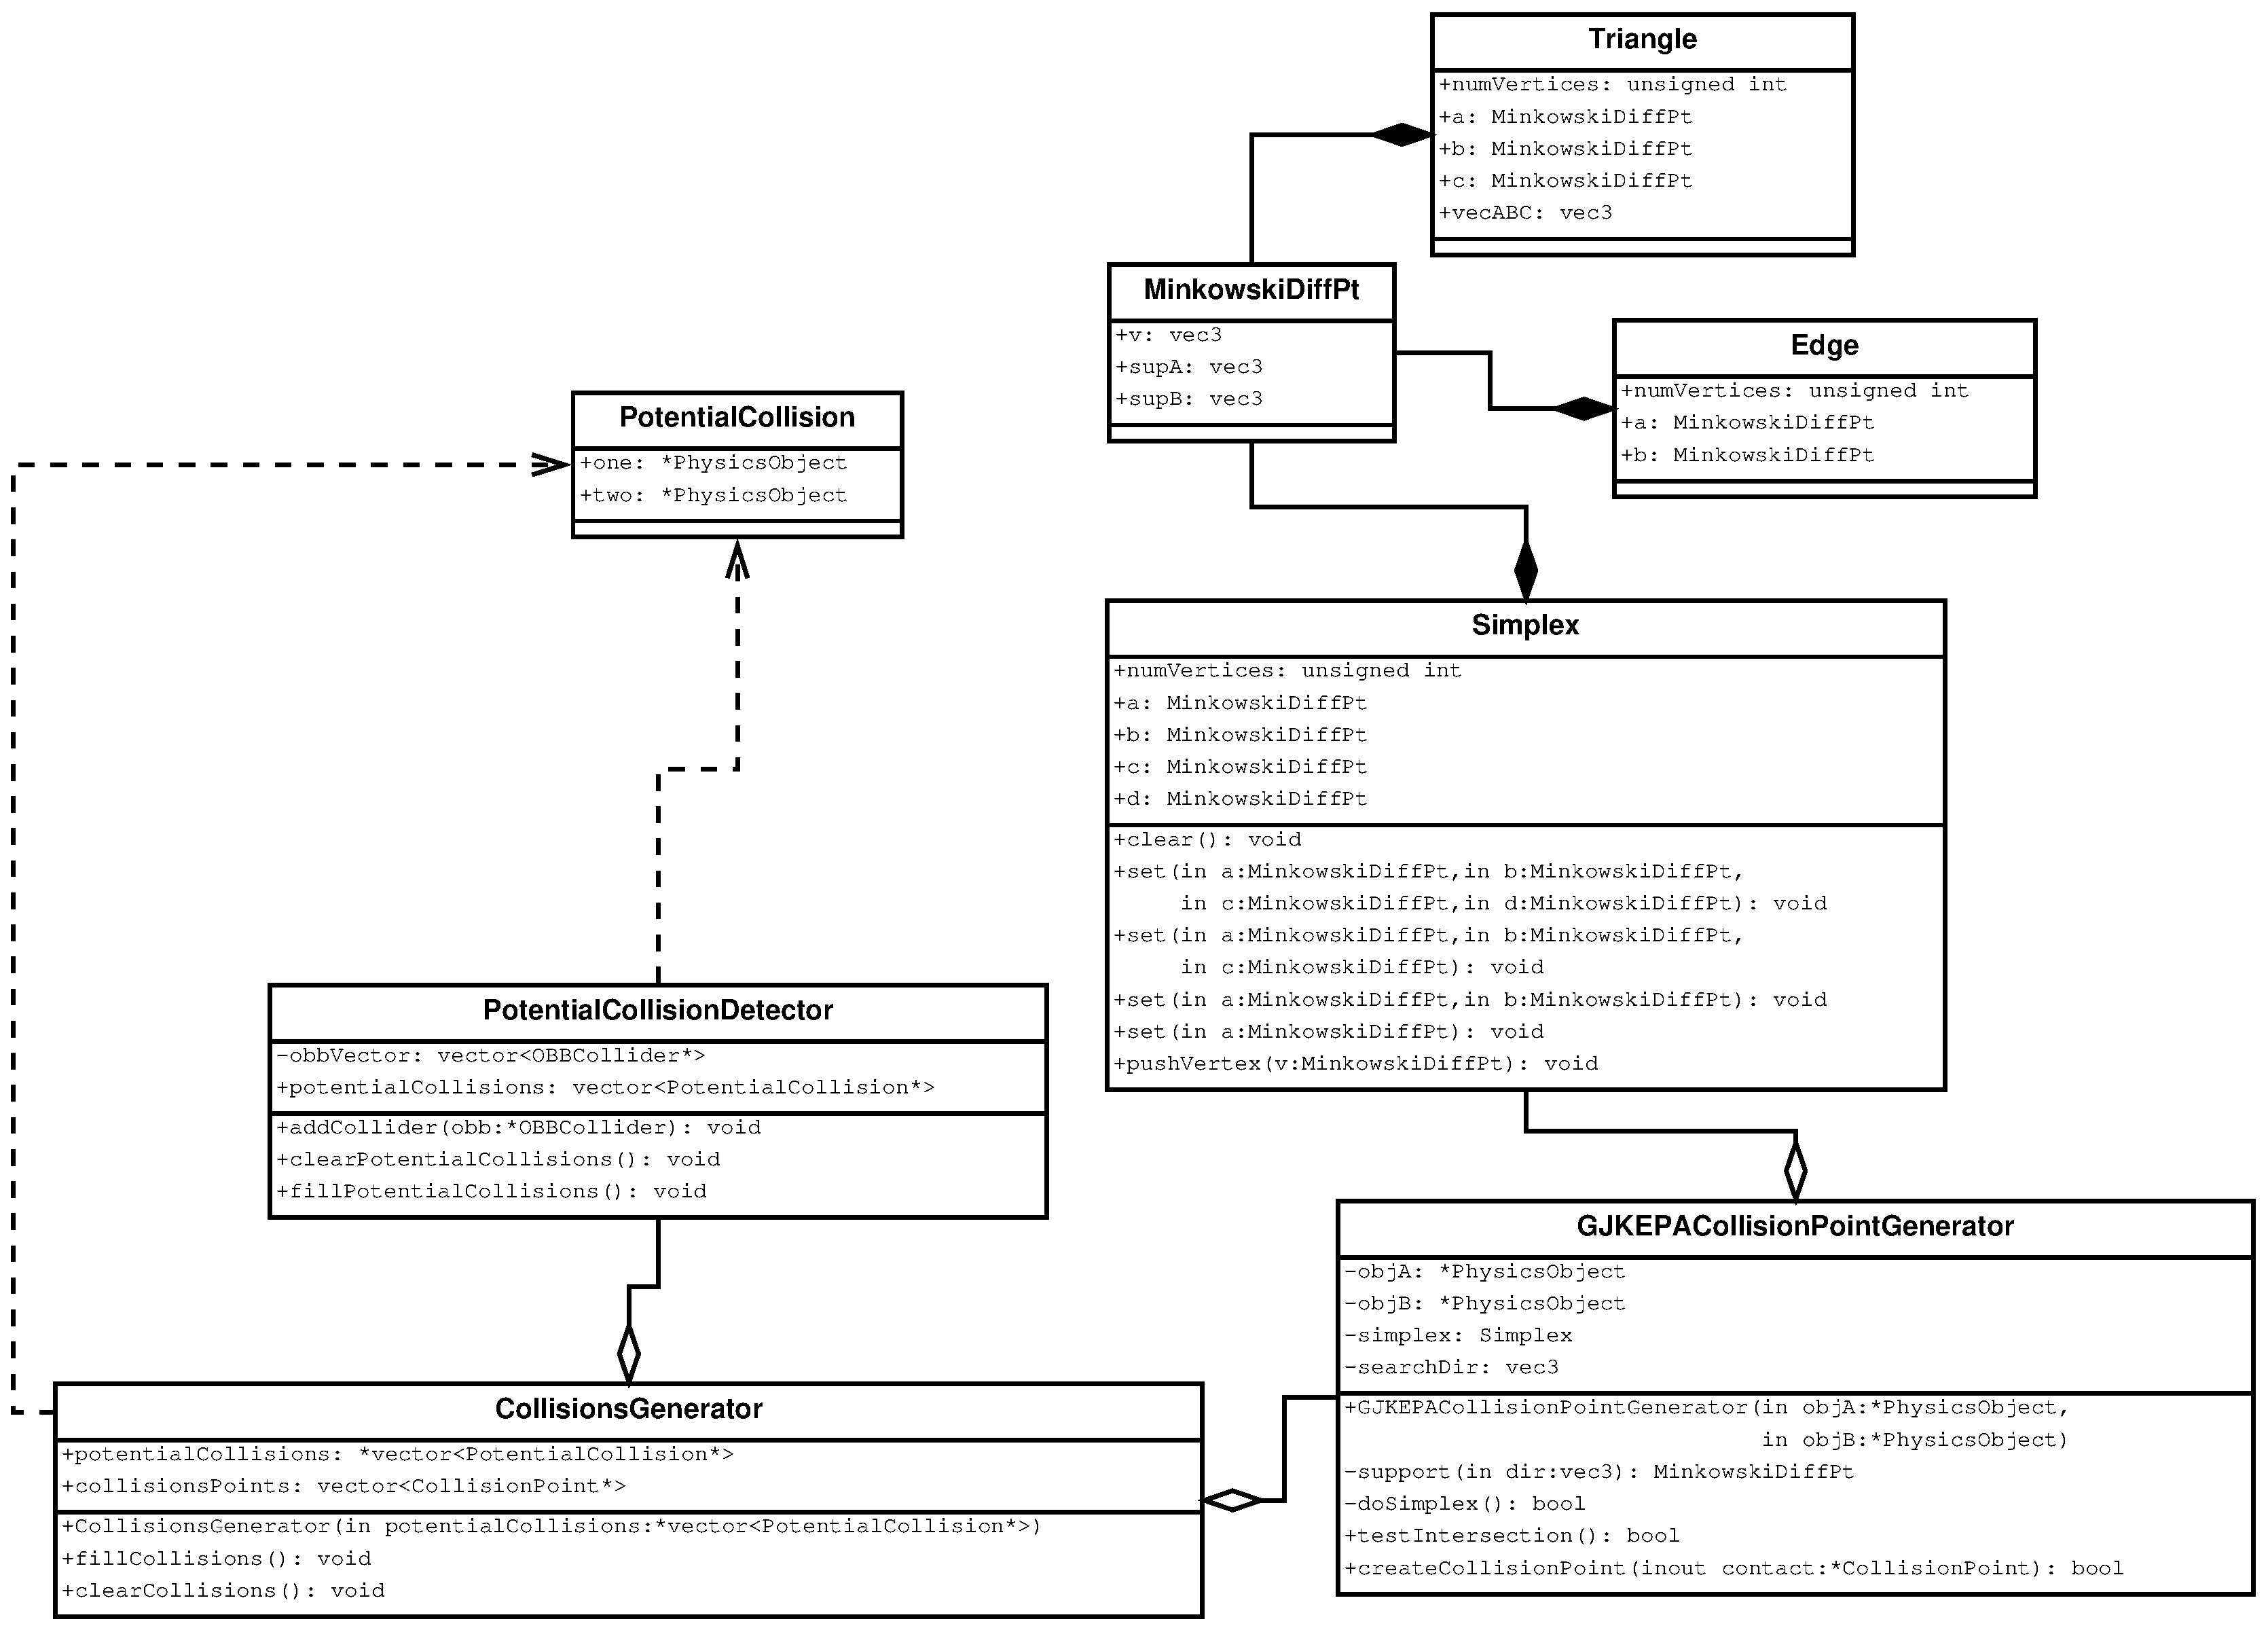
\includegraphics[width=1.0\linewidth]{pics/CollisionDetection.eps}
	\caption[]{Subsistemul de detecție de coliziuni}
	\label{fig:CollisionDetection}
\end{figure}
\end{appendices}
\end{document}
